\chapter{Introduction}
 
The use of logics has always had an important place in various sciences,
especially in~computer science and, in particular, formal verification. The
expressiveness of logics allows us to specify verified systems in a~very natural
and intuitive way without the need of deep knowledge of the used verification
procedures. The logic used range from plain propositional logic through all
kinds of first-order logics like Presburger arithmetic~\cite{presburger},
separation logic, and all the way to the more complex monadic second-order
logics, like WS$k$S~\cite{wsks}. However, with great expressiveness comes great
complexity of decision procedures of these logics, ranging from NP-complete for
propositional logic, through PSPACE-complete for quantified Boolean formulae,
with some stronger logics not being decidable at all.

WS$k$S stands for \emph{weak monadic second-order logic of $k$ successors}.
Roughly, this means that it allows to quantify over finite set variables where
every element from the universe of discourse has $k$ successors. This properties
open ways for expressing various $k$-ary tree structures, e.g. binary trees or
heaps, and linear structures, e.g. linked lists, as well. Decision procedures
for WS$k$S are usually based on the correspondence between WS$k$S formulae and
languages of finite automata (be it word or tree automata). The atomic
subformulae of an
examined WS$k$S formula $\phi$ are translated to finite (word/tree)
automata, which are further connected or manipulated using automata manipulation
techniques according to the structure of $\phi$. The resulting automaton then
represents the language encoding all models of $\phi$. The problem of checking
satisfiability (unsatisfiability/validity/invalidity) of $\phi$ is in the
NONELEMENTARY complexity class~\cite{wsksisnonelementary}. The main source of
this complexity is the occurence of quantifier alternations in $\phi$. In the
automata construction each quantifier alternation yields projection and
complementation of the automaton, for which there is currently no known
algorithm other than exponential.

There has been several attempts to implement a~decision procedure for WS$k$S,
like~\cite{nfa} for $k = 1$. Currently the best one is the tool
\textsc{MONA}~\cite{mona-tacas}, an implementation of an~automata-based decision
procedure which is quite fast and uses deterministic finite word and binary
bottom-up tree automata for deciding WS1S and WS2S formulae respectively. The
authors of \textsc{MONA} have developed a~number of heuristics, such as the use
of binary decision diagrams for the representation of transition functions of
automata or cache-friendly implementation of hash tables that made \textsc{MONA}
perform well on many practical examples in spite of the terrifying worst-case
complexity. However, there still remains a large class of practical examples for
which \textsc{MONA} fails.
\newpage
Recently, there has been a~major advance in the algorithms manipulating
non-deter\-mi\-ni\-stic automata (like~\cite{vata}). Even problems with high
worst-case complexity like testing universality or language inclusion of
the automaton can now be solved efficiently in many practical cases using
algorithms that heuristically prune the search space, such as algorithms based
on antichains or on the simulation relation among states of automata.

This text describes the design and implementation of a~new decision
procedure for WS$k$S that uses non-deterministic tree automata while exploiting
the techniques for their efficient manipulation to achieve better performance.

Tha main idea of the decision procedure is to transform a WS$k$S formula $\phi$
into equivalent formula in the form of $\phi' =
\neg\exists\mathcal{X}_n\neg\ldots\neg\exists\mathcal{X}_1:\,\psi$, where $\psi$
(called the \emph{matrix}) is a~quantifier free formula constructed over atomic
formulae and their negations, using only propositional connectives $\wedge$ and
$\vee$. The procedure then constructs the automaton $\mathcal{A}_\psi$ corresponding to
$\psi$ and checks satisfiability of $\phi'$ while working only with
$\mathcal{A}_\psi$ without explicitly constructing the automaton for $\phi'$.

The rest of this thesis is organized as follows. In Chapter \ref{preli} all
necessary preliminaries are defined. A~short introduction to the theory of
formal languages will describe finite word and tree automata, as well as some
properties of their languages. Another structure that will be defined there will
be Binary Decision Diagrams, or BDDs for short, and their extensions. Chapter
\ref{wsks} defines the syntax and semantics of the WS$k$S logic and its restricted
forms. A brief description of the correspondence between tree automata and
WS$k$S formulae also appears there.
Chapter \ref{monachap} describes the approach of \textsc{MONA} and all the known
tweaks and secrets that were used during its development. In Chapter \ref{our}
our approach to a~decision procedure for the WS$k$S logic using
non-deterministic automata and its antichain-based principle will be outlined.
A~short introduction to antichain-based procedures and universality testing of
finite word and tree automata is described there as well. Chapter \ref{impl}
describes the implementation of the designed algorithm as well as some
used optimizations. The implementation is then
evaluated in Chapter \ref{evalChapter} and compared with \textsc{MONA} in
various aspects like
the speed time or the size of the generated state space.
Chapter \ref{summary} summarizes this thesis.

\chapter{Preliminaries}\label{preli}

 \section{Formal Languages}

 We define an \emph{alphabet} as a~finite non-empty set of elements called
 \emph{symbols}. A~\emph{word} over the alphabet $\Sigma$ is a~finite sequence
 $a_1a_2\ldots a_n$, such that $a_i \in \Sigma$, for all $1 \leq i \leq n$. The
 \emph{empty sequence} of symbols, i.e. a~sequence  which does not contain any
 symbols, is denoted as $\epsilon$.

Let $x = a_1a_2\ldots a_n$ and $y = b_1b_2\ldots b_m$ be words over the alphabet
$\Sigma$, for some $n, m \in \mathbb{N}$. The \emph{concatenation} of words $x$
and $y$ is defined as the word $xy = a_1a_2\ldots a_nb_1b_2\ldots b_m$. Note
that $\epsilon x = x \epsilon = x$.

Let $\Sigma$ be an alphabet. We denote the set of all words over $\Sigma$ as
$\Sigma^*$. The set of all words except for the empty word is denoted as
$\Sigma^+ = \Sigma^* \setminus \{\epsilon\}$. We call $L \subseteq \Sigma^*$
a~\emph{language} over $\Sigma$.

 \section{Finite Automata}

 A~\emph{non-deterministic finite} (word) \emph{automaton} (further abbreviated
 as FA) is a~quintuple $\mathcal{A} = (Q, \Sigma, \delta, I, F)$, where
  \begin{itemize}
\item $Q$ is a~finite set of \emph{states},  
\item $\Sigma$ is the input alphabet, \item $\delta$ $ \subseteq Q
\times\Sigma\times Q$ is the transition relation. We use $p
\overset{a}{\longrightarrow} q$, for $p, q \in Q$ and $a \in \Sigma$ to denote
that $(p, a, q) \in \delta$,
\item $I$ $ \subseteq Q$ is the set of \emph{initial states}, 
\item $F$ $ \subseteq Q$ is the set of \emph{final states}.
	\end{itemize}
	
	Further we call a~set of states in $\mathcal{A}$, i.e. a~subset of $Q$, a
\emph{macro-state} and we define the post-image of a~state~$p$ as
$Post(p) = \{p'\in Q \mid \exists a \in \Sigma: (p, a, p') \in \delta\}$.
	
Let $\mathcal{A} = (Q, \Sigma, \delta, I, F)$ be a~FA. A~\emph{run} of
$\mathcal{A}$ over the word $w = a_1a_2\ldots a_n \in \Sigma^*$ from the state
$p \in Q$ to the state $r \in Q$ is a~sequence of states $q_0q_1\ldots q_n$,
such that $q_0 = p, q_n = r$ and for all $1 \leq i \leq n$ there is a~transition
$q_{i-1} \overset{a_i}{\longrightarrow} q_i$ in $\delta$. We write $p
\overset{w}{\Longrightarrow} r$ to denote that there exists a~run from the state
$p$ to the state $r$ over the word $w$.
\newpage
The \emph{language} accepted by a~state $q \in Q$ is defined as
$L_{\mathcal{A}}(q) = \{w \mid q \overset{w}{\Longrightarrow} q_f, q_f \in F\}$.
If it is clear which FA $\mathcal{A}$ we are referring to, we can simplify
this to $L(q)$. The language accepted by a~set of states $S \subseteq
Q$ is further defined as $L_{\mathcal{A}}(S) = \bigcup_{q \in S}
L_{\mathcal{A}}(q)$ and the language accepted by the automaton $\mathcal{A}$ is
defined as $L(\mathcal{A}) = L_{\mathcal{A}}(I)$.
	
A~\emph{deterministic finite automaton} (DFA) is a~FA $\mathcal{A}$ where $|I| =
1$ and $\forall q \in Q, \forall a~\in~\Sigma: |\{ r \in Q \mid q
\overset{a}{\longrightarrow} r\}| \leq 1$, i.e. $\delta$ is a~partial function
$\delta : Q \times \Sigma \longrightarrow Q$. If $\delta$ is total, i.e.
$\forall q \in Q, \forall a \in \Sigma : |\delta(q, a)| = 1$, we call
$\mathcal{A}$ a~\emph{complete deterministic finite automaton}. It can be shown
that for every deterministic FA there exists a~language equivalent complete
deterministic FA, by adding a~new non-final sink state.
	
	\begin{lemma}
For every non-deterministic finite automaton $\mathcal{A}$, there exists a
deterministic finite automaton $\mathcal{A}'$ such that $L(\mathcal{A}) =
L(\mathcal{A}')$.
	\end{lemma}
	
	\begin{proof}
	Let $\mathcal{A} = (Q, \Sigma, \delta, I, F)$ be a~FA. We can construct
	the DFA $\mathcal{A}'= (Q', \Sigma, \delta', I', F')$, such that
	$L(\mathcal{A}) = L(\mathcal{A}')$, by the following method:
	\begin{eqnarray*}
	 Q' & = & 2^Q,\\
	 \delta' & = & \{S \overset{a}{\longrightarrow} R \mid S \in 2^Q, R = \{r \mid
	 \exists s \in S:\,s \overset{a}{\longrightarrow} r\}\},\\
	 I' & = & \{I\},\\
	 F' & = & \{S \in 2^Q \mid S~\cap F \neq \emptyset\}.
	\end{eqnarray*}
	
	Note that $\mathcal{A}'$ is complete. It can be proved that $L(\mathcal{A}) =
	L(\mathcal{A}')$ by showing that $L(\mathcal{A}) \subseteq L(\mathcal{A}')$ and simultaneously $L(\mathcal{A}')
	\subseteq L(\mathcal{A})$~\cite{tin}.
	\end{proof}
	
	\begin{defz}
We define the class of regular languages $\mathcal{L}_R$ as the class of
languages $L \in \Sigma^*$ such that there exists a~finite automaton
$\mathcal{A}$ such that $L(\mathcal{A}) = L$.
	\end{defz}
	
	\noindent\hrulefill
	\begin{example}
	Consider the encoding of subsets of $\{1,\ldots,n\}$, for some $n \in
	\mathbb{N}$, as binary strings $X = a_1\ldots a_n$, where $a_i$ is $1$ if $i \in X$ and $0$ if
	$i \notin X$. We can construct the automaton $\mathcal{A}$ that accepts the
	encoding of the set difference $X$ of two sets $Y$ and $Z$, i.e. $X = Y
	\setminus Z$, as depicted in Figure \ref{set-automaton}.
	
	\begin{figure}[h!]
	\begin{center}
	 \scalebox{1}{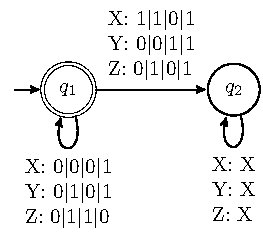
\includegraphics{fig/word-automaton-setminus.pdf}}
	 \end{center}
	 \caption{Automaton $\mathcal{A}$ accepting the encoding of the set difference
	 of a pair of sets. Note that we use the symbol $\overline{X}$ as
	 don't-care symbol, i.e. it can stand for any symbol
	 from $\Sigma$.}\label{set-automaton}
	\end{figure}
	\end{example}
	
	\noindent\hrulefill
	\newpage
 \subsection{Closure Properties of Regular Languages}

\begin{theorem}
 The class of regular languages is closed under union.
\end{theorem}

\begin{proof}
Let $\mathcal{A} = (Q_\mathcal{A}, \Sigma, \delta_\mathcal{A}, I_\mathcal{A},
F_\mathcal{A})$ and $\mathcal{B} = (Q_\mathcal{B}, \Sigma, \delta_\mathcal{B},
I_\mathcal{B}, F_\mathcal{B})$ be a~pair of finite automata such that
$Q_\mathcal{A} \cap Q_\mathcal{B} = \emptyset$. We construct an automaton
$\mathcal{A} \cup \mathcal{B}$ accepting the \emph{union} of languages
$L(\mathcal{A})$ and $L(\mathcal{B})$: 
\begin{equation} \mathcal{A} \cup \mathcal{B} = (Q_\mathcal{A} \cup
 Q_\mathcal{B}, \Sigma, \delta_\mathcal{A} \cup \delta_\mathcal{B},
 I_\mathcal{A} \cup I_\mathcal{B}, F_\mathcal{A} \cup
F_\mathcal{B}).
\end{equation}

\noindent The proof that $L(\mathcal{A} \cup \mathcal{B}) = L(\mathcal{A}) \cup
L(\mathcal{B})$ can be found for example in~\cite{tin}.
\end{proof}

  \begin{theorem}
	 The class of regular languages is closed under intersection.
	\end{theorem}
	
	\begin{proof}
Let $\mathcal{A} = (Q_\mathcal{A}, \Sigma, \delta_\mathcal{A}, I_\mathcal{A},
F_\mathcal{A})$ and $\mathcal{B} = (Q_\mathcal{B}, \Sigma, \delta_\mathcal{B},
I_\mathcal{B}, F_\mathcal{B})$ be a~pair of finite automata. We construct an
automaton $\mathcal{A} \cap \mathcal{B}$ accepting the \emph{intersection} of
languages $L(\mathcal{A})$ and $L(\mathcal{B})$:
\begin{equation}
\mathcal{A} \cap \mathcal{B} = (Q_\mathcal{A} \times
Q_\mathcal{B}, \Sigma, \delta, I_\mathcal{A} \times I_\mathcal{B}, F_\mathcal{A}
\times F_\mathcal{B})
\end{equation} where 
\begin{equation}
\delta = \{(p_1, p_2) \overset{a}{\longrightarrow} (q_1, q_2) \mid p_1
\overset{a}{\longrightarrow} q_1 \in \delta_{\mathcal{A}} \wedge p_2
\overset{a}{\longrightarrow} q_2 \in \delta_{\mathcal{B}}\}.
\end{equation}

\noindent The proof that $L(\mathcal{A} \cap \mathcal{B}) = L(\mathcal{A}) \cap
L(\mathcal{B})$ can be found for example in~\cite{tin}.
\end{proof}
	
 \begin{theorem}
  The class of regular languages is closed under language complementation.
\end{theorem}
	
	\begin{proof}
Let $\mathcal{A} = (Q_\mathcal{A}, \Sigma, \delta_\mathcal{A}, I_\mathcal{A},
F_\mathcal{A})$ be a~complete deterministic FA. We construct an automaton
accepting the \emph{complement} of $L(\mathcal{A})$:
\begin{equation}
\overline{\mathcal{A}} =
(Q_\mathcal{A}, \Sigma, \delta_\mathcal{A}, I_\mathcal{A}, Q_\mathcal{A}
\setminus F_\mathcal{A}).
\end{equation}
	
\noindent The proof that $L(\overline{\mathcal{A}}) = \Sigma^* \setminus
L(\mathcal{A})$ can be found for example in~\cite{tin}.
 \end{proof}

 \section{Tree Automata}

 A~\emph{ranked alphabet} $\Sigma$ is a~finite set of symbols together with a
 ranking function $\#: \Sigma \to \mathbb{N}$, we call $\#a$ the \emph{rank}
 of $a$. For any $n \geq 0$, we denote by $\Sigma_n$ the set of all symbols of rank
 $n$ from $\Sigma$. We denote by $\epsilon \in \mathbb{N}^*$ the \emph{empty
 sequence}.

Then a~\emph{tree} $t$ over a~ranked alphabet $\Sigma$ is defined as a~partial
mapping $t : \mathbb{N}^* \to \Sigma$, that satisfies the following conditions:
 \begin{enumerate}
  \item \emph{dom}($t$) is a~finite prefix-closed subset of $\mathbb{N}^*$,
  \item for every $v \in dom(t)$, called a~\emph{node} of $t$, the following
holds: $(\#t(v) = n \geq 0) \Longrightarrow$\\ $\{i \mid vi \in dom(t)\} =
\{1,\ldots,n\}$.
 \end{enumerate}

For a~node $v$, the $i$-th \emph{child} of $v$ is the node $vi$, and the $i$-th
\emph{subtree} of $v$ is the tree $t'$ such that for all $v' \in \mathbb{N}^*$, 
$t'(v') = t(viv')$. A~node $v$ which does not have any children is called a
\emph{leaf} of the tree $t$. The set of all trees over the alphabet $\Sigma$ is
denoted as $T_\Sigma$.
\newpage
A~(finite, non-deterministic) \emph{tree automaton} (further abbreviated as TA)
is a~quadruple $\mathcal{A} = (Q, \Sigma, \delta, F)$, where:
 \begin{itemize}
   \item $Q$ is a~finite set of \emph{states},
	\item $\Sigma$ is a~\emph{ranked alphabet},
	\item $\delta$ is the \emph{set of transitions},
	\item $F$ $ \subseteq Q$ is the set of \emph{final states}.
 \end{itemize}

Each transition is defined as a~triple $((q_1,\ldots,q_n), a, q)$, where
$q_1,\ldots,q_n,q \in Q, a \in \Sigma$ and $\#a = n$. We use equivalently
$(q_1,\ldots,q_n) \overset{a}{\longrightarrow} q$ and $q
\overset{a}{\longrightarrow}  (q_1,\ldots,q_n)$ to denote that
$((q_1,\ldots,q_n), a, q) \in \delta$, for \emph{bottom-up} and \emph{top-down}
representation respectively. In the special case where $n = 0$, we speak about
the so-called \emph{leaf rules} that can be abbreviated as
$\overset{a}{\longrightarrow}  q$ or $q \overset{a}{\longrightarrow} $.

Let $\mathcal{A} = (Q, \Sigma, \delta, F)$ be a~TA. We define a~\emph{run} of
$\mathcal{A}$ over a~tree $t \in T_\Sigma$ as a~mapping $\varphi: dom(t) \to Q$
such that for each node $v \in dom(t)$ of rank $\#t(v) = n$, where $\varphi(v) =
q$, if $\varphi(vi) = q_i$ for all $1 \leq i \leq n$, then $(q_1,\ldots,q_n)
\overset{t(v)}{\longrightarrow} q$. We write $t
\overset{\varphi}{\Longrightarrow} q$ to denote that $\varphi$ is a~run of
$\mathcal{A}$ over $t$ such that $\varphi(\epsilon) = q$. We write $t
\Longrightarrow q$ to denote that there exists a~run $\varphi$ for which $t
\overset{\varphi}{\Longrightarrow} q$.

The \emph{language} accepted by a~state $q$ is defined as $L_{\mathcal{A}}(q) =
\{t \mid t \Longrightarrow q\}$. For a~set of states $S \subseteq Q$ we define
the language accepted by this set as $L_{\mathcal{A}}(S) = \bigcup_{q \in S}
L_{\mathcal{A}}(q)$. Similarly to FA, if it is clear which TA $\mathcal{A}$ we
are referring to, we only write $L(q)$ or $L(S)$. Then language of $\mathcal{A}$
is defined as $L(\mathcal{A}) = L_{\mathcal{A}}(F)$.

\begin{defz}
A~\emph{deterministic finite tree automaton} (abbreviated as DTA) is a
TA such that there are no two rules with the
same left-hand, or right-hand, side in $\delta$ for bottom-up DTA or top-down
DTA respectively.
\end{defz}

Note that the expressive power of bottom-up and top-down NTA is the same.
However, top-down DTA are strictly less powerful than top-down NTA.
See~\cite{tata} for more details.

\begin{defz}
We define the class of regular tree languages $\mathcal{L}$ as the class of
languages $L \subseteq T_\Sigma$ such that there exists a~finite tree automaton
$\mathcal{A}$ such that $L(\mathcal{A}) = L$.
\end{defz}

%%% REGULAR TREE LANGUAGES

%%% BOTTOM UP DETERMINISTIC TREE AUTOMATA

\subsection{Closure Properties of Regular Tree Languages}\label{ta-closures}

\begin{theorem}
 The class of regular tree languages is closed under intersection.
\end{theorem}

\begin{proof}
Let $\mathcal{A} = (Q_\mathcal{A}, \Sigma, F_\mathcal{A}, \delta_\mathcal{A})$
and $\mathcal{B} = (Q_\mathcal{B}, \Sigma, F_\mathcal{B}, \delta_\mathcal{B})$
be two tree automata. We construct a~tree automaton $\mathcal{A} \cap
\mathcal{B}$ accepting the \emph{intersection} of languages $L(\mathcal{A})$ and
$L(\mathcal{B})$:
\begin{equation}
\mathcal{A} \cap \mathcal{B}
= (Q_\mathcal{A} \times Q_\mathcal{B}, \Sigma, F_\mathcal{A} \times
F_\mathcal{B},\delta) \end{equation} where
 \begin{align}
 \delta = &\{
 ((q^1_1,q^2_1),\ldots,(q^1_n,q^2_n)) \overset{f}{\longrightarrow} (q^1,
 q^2)\nonumber \\
  & \mid (q^1_1,\ldots,q^1_n) \overset{f}{\longrightarrow} q^1 \in
  \delta_{\mathcal{A}} \wedge (q^2_1,\ldots,q^2_n) \overset{f}{\longrightarrow}
  q^2 \in \delta_{\mathcal{B}})\}.
	\end{align}
\end{proof}

Note that this construction preserves determinism, i.e. if the two given
automata are deterministic, then so is the product automaton.
\begin{theorem}
 The class of regular tree languages is closed under union.
\end{theorem}

\begin{proof}
Let $\mathcal{A} = (Q_\mathcal{A}, \Sigma, F_\mathcal{A}, \delta_\mathcal{A})$
and $\mathcal{B} = (Q_\mathcal{B}, \Sigma, F_\mathcal{B}, \delta_\mathcal{B})$
be two tree automata. We construct a~tree automaton $\mathcal{A} \cup
\mathcal{B}$ accepting the \emph{union} of languages $L(\mathcal{A})$ and
$L(\mathcal{B})$:
\begin{equation}
\mathcal{A} \cup
\mathcal{B} = (Q_\mathcal{A} \cup Q_\mathcal{B}, \Sigma, F_\mathcal{A} \cup
F_\mathcal{B}, \delta_\mathcal{A} \cup \delta_\mathcal{B}).
\end{equation}
\end{proof}

\begin{theorem}
 The class of regular tree languages is closed under language complementation.
\end{theorem}

\begin{proof}
Let $\mathcal{A} = (Q, \Sigma, F, \delta)$ be a~complete bottom-up deterministic
TA. We construct a~tree automaton accepting the \emph{complement} of the
language $L(\mathcal{A})$:
\begin{equation}
\overline{\mathcal{A}} = (Q, \Sigma, Q \setminus F, \delta).
\end{equation}
\end{proof}

Note that for non-deterministic tree automata there is currently known no
complementation procedure better than first bottom-up determinizing the
automaton and then complementing it using the construction above.

 \subsection{Relations on Trees}

Given a~ranked alphabet $\Sigma$ and $n \geq 0$, let $(T_\Sigma)^n$ be the
\emph{Cartesian product} $T_\Sigma \times (T_\Sigma)^{n-1}$ with the ground case
$(T_\Sigma)^0 = \{\top\}$, where $\{\top\}$ is a~neutral element w.r.t.\ 
Cartesian product. A~subset of $(T_\Sigma)^n$ is an $n$-ary relation on
$T_\Sigma$. Further, let $\Sigma^n_\bot$ be the \emph{compound alphabet}
$\Sigma_\bot^n = (\Sigma \cup \{\bot\})^n$ where $\bot$ is a~new symbol such
that $\bot \notin \Sigma$ and $\#\bot = 0$. We write the symbol
$(f_1,\ldots,f_n)$ of $\Sigma_\bot^n$ as $f_1\ldots f_n$. Arities of symbols in
$\Sigma_\bot^n$ are defined as $\#(f_1\ldots f_n) =
\text{max}(\#f_1,\ldots,\#f_n)$.

Let $[\cdot]$ be a~function that maps $n$-tuples of trees over $T_\Sigma$ to
trees over $T_{\Sigma_\bot^n}$:
\begin{equation}
    [\cdot] :
    \begin{cases}
     (T_\Sigma)^n \rightarrow T_{\Sigma^n_\bot}\\
		 f_1(t_1^1,\ldots,t^{\#f_1}_1),\ldots,f_n(t_n^1,\ldots,t^{\#f_n}_n) \mapsto\\
		 \ \ f_1\ldots f_n([t_1^1,\ldots,t_n^1],\ldots,[t_1^m,\ldots,t_n^m])
   \end{cases}
\end{equation}
 where $m$ is the maximal arity of $f_1,\ldots,f_n \in \Sigma$ and $t_i^j$ is,
 by convention, $\bot$ when $j > \#f_i$.

\begin{defz}
Rec, for recognizable tree relations, is the class of relations $R \subseteq
(T_\Sigma)^n$ such that the language 
\begin{equation}
\{[t_1,\ldots,t_n] \mid (t_1,\ldots,t_n)
\in R\}
\end{equation} is accepted by a~tree automaton on the alphabet $\Sigma_\bot^n$.
\end{defz}

\begin{prop}
Rec is closed under Boolean operations, i.e. intersection, union and
complementation.
\end{prop}

\begin{proof}
This is due to closure properties of tree automata (see Section
\ref{ta-closures}).
\end{proof}

\begin{defz}
If $R \subseteq (T_\Sigma)^n$ where $n \geq 1$ and $1 \leq i \leq n$, then the
$i$-th \emph{projection} of R is the relation $R_i \subseteq (T_\Sigma)^{n-1}$
defined as follows: 
\begin{equation}
 R_i(t_1,\ldots,t_{n-1}) \Leftrightarrow \exists t \in T_\Sigma
.\ R(t_1,\ldots,t_{i-1},t,t_i,\ldots,t_{n-1}).
\end{equation}
\end{defz}

\begin{lemma}
Rec is closed under projection.
\end{lemma}

\begin{proof}
 Let us assume that $R \in Rec$. The $i$-th projection $R_i$ of $R$ is simply
 its image by the following tree homomorphism:
 \begin{equation}
 h_i(f_1\ldots f_n (t_1,\ldots,t_k)) \overset{\mathit{def}}{=} f_1\ldots f_{i-1}f_{i+1}\ldots f_n(h_i(t_1),\ldots,h_i(t_m))
\end{equation}
where $m$ is the arity of $(f_1\ldots f_{i-1}f_{i+1}\ldots f_n)$, which is
smaller or equal to $k$. Because linear homomorphisms preserve recognizability
(Theorem 1.4.3 in~\cite{tata}), $R_i \in Rec$.
\end{proof}

\begin{defz}
 If $R \subseteq (T_\Sigma)^n$ where $n \geq 0$ and $1 \leq i \leq n+1$ then the
 $i$-th \emph{cylindrification} of R is the relation $R_i \subseteq
 (T_\Sigma)^{n+1}$ defined as follows: 
\begin{equation}
 R^i(t_1,\ldots,t_{i-1},t,t_i,\ldots,t_n)
 \Leftrightarrow R(t_1,\ldots,t_{i-1},t_i,\ldots,t_n).
\end{equation}
\end{defz}

\begin{lemma}
Rec is closed under cylindrification.
\end{lemma}

\begin{proof}
 Similarly to projection, $i$-th cylindrification is obtained as an inverse
 homomorphic image, and thus is recognizable as stated by Theorem 1.4.4. in~\cite{tata}.
\end{proof}

 \section{Binary Decision Diagrams}\label{bdd}

We define a~\emph{Boolean function} of \emph{arity} $k$ as a~function $f :
\{0,1\}^k \to \{0,1\}$. A \emph{reduced ordered binary decision
diagram} (abbreviated as ROBDD or just BDD) $r$ over a~set of $n$ Boolean
variables $X = \{x_1,\ldots,x_n\}$ is a~connected directed acyclic graph with a
single \emph{source node} called \emph{root} and at least one of two sink nodes
0 and 1. Nodes that are not sink nodes are called \emph{internal nodes}.
Assignment of Boolean variables to each of the internal nodes is done by the
function $\mathit{var}$. We assume that $X$ is ordered in the following way:
$x_1 < x_2 < \ldots < x_n$.
For every internal node $v$, there exists two outgoing edges labeled as $low$
and $\mathit{high}$, such that $\mathit{var}(v) < \mathit{var}(v.low) \wedge \mathit{var}(v) <
\mathit{var}(v.high)$; and $v.low \neq v.high$ as well (since otherwise it could be further reduced).

Nodes of a~BDD represent $n$-ary Boolean functions that map each assignment to
the Boolean variables in $X$ to a~corresponding Boolean value defined as
follows, using $\overline{x}$ as an~abbreviation for $x_1\ldots x_n$:
\begin{eqnarray*}
 \text{\textlbrackdbl} 0\text{\textrbrackdbl} & = & \lambda\overline{x}.0\\
 \text{\textlbrackdbl} 1\text{\textrbrackdbl} & = & \lambda\overline{x}.1\\
 \text{\textlbrackdbl} v\text{\textrbrackdbl} & = & \lambda\overline{x}.(\neg
 x_i \wedge \text{\textlbrackdbl} v.low\text{\textrbrackdbl}(\overline{x})) \vee
 (x_i \wedge \text{\textlbrackdbl} v.high\text{\textrbrackdbl}(\overline{x}))\\
       & \text{where} & \mathit{var}(v) = x_i
\end{eqnarray*}
We can further extend the notion of these functions to an arbitrary nonempty
codomain $S$, $f : \{0,1\}^k \longrightarrow
S$.
The notion of ROBDDs can then be further generalized to \emph{multi-terminal
binary decision diagrams} (abbreviated as MTBDDs), which is essentially the same data
structure as a BDD, with the only difference being the fact that the set of
sink nodes is not restricted to only two nodes but to any number of sink nodes
labelled by elements of $S$. All standard notions for ROBDDs can be naturally
extended to MTBDDs.

A \emph{shared} MTBDD $s$ is a~MTBDD with multiple source nodes (or roots) that
represent a~mapping of every element of the set of roots $R$ to a~function
induced by the MTBDD corresponding to the given root. We can see the difference
between MTBDDs and BDDs in the Figure \ref{mtbdd-vs-bdd}.

\begin{figure}
\begin{subfigure}{.5\textwidth}
  \centering
  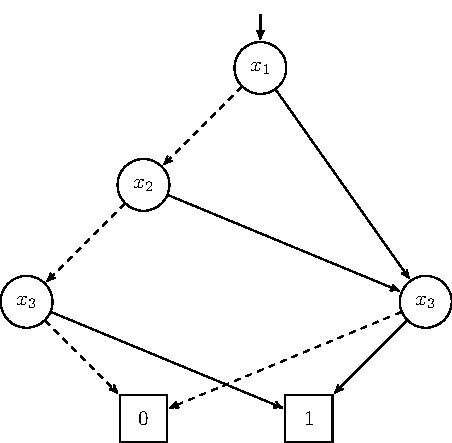
\includegraphics[width=.7\linewidth]{fig/bdd}
  \caption{BDD}
  \label{BDD}
\end{subfigure}%
\begin{subfigure}{.5\textwidth}
  \centering
  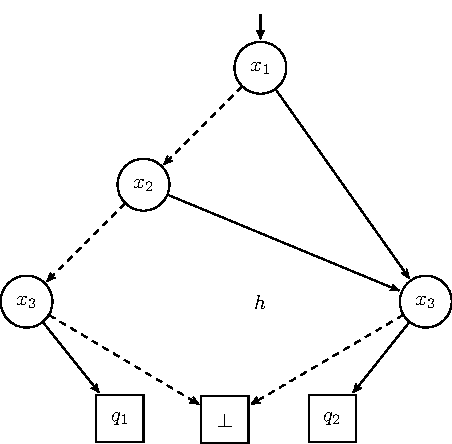
\includegraphics[width=.7\linewidth]{fig/mtbdd}
  \caption{MTBDD}
  \label{MTBDD}
\end{subfigure}
\caption{Difference between BDD and MTBDD.}
\label{mtbdd-vs-bdd}
\end{figure}

For manipulation with BDDs $f$, $g$ we define the $\mathit{Apply}_1$ function
for some unary leaf operator $\mathit{op}_1$ and the $\mathit{Apply}_2$ function for some
binary leaf operator $\mathit{op}_2$ as follows: 
\begin{eqnarray}
\mathit{Apply}_1(f,\mathit{op}_1) & = & \lambda
\overline{x}\,.\,\mathit{op}_1(\text{\textlbrackdbl}f(\overline{x})\text{\textrbrackdbl}),\\
\mathit{Apply}_2(f, g, \mathit{op}_2) & = & \lambda
\overline{x}\,.\,\mathit{op}_2(\text{\textlbrackdbl}f(\overline{x})\text{\textrbrackdbl}, \text{\textlbrackdbl}g(\overline{x})\text{\textrbrackdbl}).
\end{eqnarray}

\newpage
\subsection[Usage
of MTBDDs with TA]{Using Shared MTBDDs for Encoding Transition Function of Tree Automata} Let $\mathcal{A} = (Q, \Sigma, \delta, F)$
be a~tree automaton, such that $\Sigma = \{0, 1\}^n$, for some $n$. Each
position $1 \leq i \leq n$ is then assigned a~Boolean variable from the set $X =
\{x_1,\ldots,x_n\}$. We use $Q^\#$ to denote the set of all tuples of states from $Q$ with up to the
maximum arity that some symbol in $\Sigma$ has.

The \emph{bottom-up} representation of the transition function $\delta$ of the
TA $\mathcal{A}$ uses a~shared MTBDD $\delta^{bu}$ over $\Sigma$, where the set
of roots $R = Q^\#$, and the domain set of values of sink nodes is $2^Q$ that
is, the MTBDD $\delta^{bu}$ represents the function \textlbrackdbl $\delta^{bu}$
\textrbrackdbl $: Q^\# \rightarrow (\Sigma \rightarrow 2^Q)$ where
 \begin{equation}
  \text{\textlbrackdbl} \delta^{bu} \text{\textrbrackdbl} =
 \lambda (q_1,\ldots,q_p)\ a . \{q \mid (q_1,\ldots,q_p)
 \overset{a}{\longrightarrow} q\}. \end{equation}

The \emph{top-down} representation of the transition function $\delta$ of the TA
$\mathcal{A}$ uses a~shared MTBDD $\delta^{td}$ over $\Sigma$, where the set of
roots $R = Q$ and the domain of labels of sink nodes is $2^{Q^\#}$. The MTBDD
$\delta^{td}$ then represents the function \textlbrackdbl $\delta^{td}$
\textrbrackdbl $: Q \rightarrow (\Sigma \rightarrow 2^{Q^\#})$ where
\begin{equation} \text{\textlbrackdbl} \delta^{td} \text{\textrbrackdbl} =
\lambda q\ a .
\{(q_1,\ldots,q_p) \mid q \overset{a}{\longrightarrow} (q_1,\ldots,q_p)\}.
\end{equation}
\noindent\hrulefill
\begin{example}
 Consider the word automaton $\mathcal{A}$ from Example
 \ref{set-automaton} accepting the encoding of set difference of two sets with
 the following transitions:
 \begin{eqnarray*}
  q_1 & \overset{00\overline{X}}{\longrightarrow} & q_1\\
  q_1 & \overset{011}{\longrightarrow} & q_1\\
  q_1 & \overset{110}{\longrightarrow} & q_1\\
  q_1 & \overset{10\overline{X}}{\longrightarrow} & q_2\\
  q_1 & \overset{010}{\longrightarrow} & q_2\\
  q_1 & \overset{111}{\longrightarrow} & q_2\\
  q_2 & \overset{\overline{X}\overline{X}\overline{X}}{\longrightarrow} & q_2
 \end{eqnarray*}
  Note that we use the symbol $\overline{X}$ to substitute either 0 or 1
  in its place. The MTBDD encoding the transition function of this
  automaton is depicted in Figure \ref{mtbdd}.
 
 \begin{figure}[h!]
  \begin{center}
   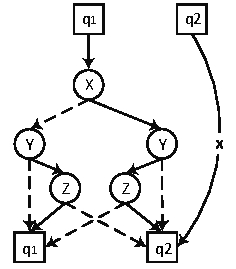
\includegraphics{fig/bdd-transition-function-encoding}
  \end{center}
  \caption{The MTBDD encoding the transition function corresponding to
  $\mathcal{A}$ from Example
  \ref{set-automaton}}\label{mtbdd}
 \end{figure}
 
\end{example}

\noindent\hrulefill

\chapter{The WS$k$S Logic}\label{wsks}
The abbreviation WS$k$S stands for \emph{weak second-order monadic logic of $k$
successors}. This means that it is a~logic that allows quantification over set
variables (second-order), which can only represent \emph{finite} sets (weak) of
elements and \emph{not functions} (monadic), over a~universe of discourse where
every element has $k$ successors, and can therefore express linear (for $k
= 1$) as well as tree (for $k \geq 2$) structures.
 
 \section{Syntax}
 A~WS$k$S \emph{term} is an empty constant $\epsilon$, a~first-order variable
 symbol written in lower-case letters (e.g. \emph{x, y, z, \ldots}) or an unary
 symbol from $\{1,\ldots,k\}$ written in postfix notation.
 For example, $x1123$ or $\epsilon2111$ are terms, where the latter can be
 shortened to $2111$.

The \emph{atomic formulae} are defined as follows:
 \begin{enumerate}
  \item For terms $s$ and $t$, the equality $s = t$ is an~atomic formula.
\item For terms $s$ and $t$, inequalities $s \leq t$ and $s \geq t$ are atomic
formulae.
\item For a~term $t$ and a~second-order variable $X$, the membership constraint
$t \in X$ is an~atomic formula.
 \end{enumerate}

A WS$k$S \emph{formula} is then built out of atomic formulae using the
classical logical connectives $\wedge, \vee, \neg, \Leftarrow, \Rightarrow,
\Leftrightarrow$ and quantifiers $\exists x, \forall x$ and $\exists X, \forall
X$ for quantification over first-order variables and second-order variables
respectively.

The syntax can be further restricted to only a~subset of logical connectives
and atomic formulae without harm to the expressive power of the logic. This will be
further explained in Section \ref{restricted}. The set of \emph{free variables}
of a~formula $\mathit{freeVars}(\psi)$ is defined as usual.
  
  \noindent\hrulefill
  \begin{example}
  The following example WS$k$S formula $\varphi$ denotes that the set $X$
  contains exactly one element from the universe of discourse:
  \begin{equation}
   \varphi(X) \overset{\mathit{def}}{=} \exists p:\,p \in X \wedge \forall r:\,
   p \neq r \Rightarrow r \not\in X
  \end{equation}
   \hrulefill
  \end{example}\label{wsks-formula}
  
  \section{Semantics}
	
We will interpret terms as strings belonging to $\{1,\ldots,k\}^*$, $=$ as the
equality of strings, and $\leq$ as the prefix ordering. Second order variables
will be interpreted as \emph{finite} subsets of $\{1,\ldots,k\}^*$ with
$\in$ as the membership predicate.
	
Let $t_1,\ldots,t_n \in \{1,\ldots,k\}^*$ and $S_1,\ldots,S_n$ be finite subsets
of $\{1,\ldots,k\}^*$. Given a~formula $\psi(x_1,\ldots,x_n,X_1,\ldots,X_m)$
with free variables $x_1,\ldots,x_n$, $X_n,\ldots,X_m$, the assignment $\delta =
\{ x_1 \mapsto t_1,\ldots, x_n \mapsto t_n, X_1 \mapsto S_1,\ldots, X_m \mapsto
S_m\}$ \emph{satisfies} $\psi$ written as $\delta \models \psi$ (or also
$t_1,\ldots, t_n, S_1,\ldots,S_m \models \psi$) if replacing the variables with
their corresponding values, the formula holds in the above model.
	
  \section{Restricting Syntax}\label{restricted}
	We are going to restrict the WS$k$S syntax to use only second-order variables.
	This can be done by considering every first-order variable as a~singleton set
	and transforming every formula to an equivalent one which does not contain any
	first-order variables. We will consider only the following atomic formulae,
	where $X$ and $Y$ are second-order variables, and build formulae over them:
	\begin{itemize}
	 \item $X \subseteq Y$,
\item $\mathit{Sing}(X)$\,---\,holds true iff $X$ is a~singleton set, \item $X
= Yi$\,---\,holds true iff $X$ and $Y$ are singleton sets $\{s\}$ and $\{t\}$
respectively and $s = ti$,
	 \item $X = \epsilon$.
	\end{itemize}
	
We can also further simplify the syntax of WS$k$S formulae by restricting
logical connectives used to build the formulae to only $\exists$, $\vee$,
$\wedge$ and $\neg$. This syntax will be called
the \emph{restricted syntax} and its satisfaction relation will be denoted as
$\models_2$.
	
	\begin{prop}
There is a~translation T from WS$k$S formulae to the restricted syntax such that
\begin{equation}
s_1,\ldots,s_n,S_1,\ldots,S_m \models
\psi(x_1,\ldots,x_n,X_1,\ldots,X_m)
\end{equation} if and only if \begin{equation}\{s_1\},\ldots,\{s_n\},S_1,\ldots,S_m \models_2
T(\psi)(X_{x_1},\ldots,X_{x_n}, X_1,\ldots,X_m).
\end{equation}

 \noindent Conversely, there is a
translation $T'$ from the restricted syntax to WS$k$S such that \begin{equation}S_1,\ldots,S_m
\models T'(\psi)(X_1,\ldots,X_m)\end{equation} if and only if \begin{equation}S_1,\ldots,S_m \models_2
\psi(X_1,\ldots,X_m).\end{equation}
	\end{prop}
	\begin{proof}
We will only present a~short sketch of the proof for this proposition. For
further details see~\cite{tata}.

We can suppose that formulae will be built only upon the atomic formulae $t \in
X$ and $s = t$ and so flatten the rest of the atomic formulae. Every first-order
variable $y$ will be mapped to a~second-order variable $X_y$ as follows:
	
	 \begin{eqnarray}
	 T(y \in X) & \overset{\mathit{def}}{=} & X_y \subseteq X\\
	 T(y = xi) & \overset{\mathit{def}}{=} &  X_y = X_xi\\
	 T(x = \varepsilon) & \overset{\mathit{def}}{=} & X_x = \varepsilon\\
	 T(x = y) & \overset{\mathit{def}}{=} & X_x = X_y\\
	 T(\psi \vee \phi) & \overset{\mathit{def}}{=} & T(\psi) \vee T(\phi)\\
	 T(\psi \wedge \phi) & \overset{\mathit{def}}{=} & T(\psi) \wedge T(\phi)\\
	 T(\neg\phi) & \overset{\mathit{def}}{=} & \neg T(\phi)\\
	 T(\exists X.\phi) & \overset{\mathit{def}}{=} & \exists X.T(\phi)\\
	 T(\exists y.\phi) & \overset{\mathit{def}}{=} & \exists X_y:\ Sing(X_y) \wedge T(\phi)
	 \end{eqnarray}
	Moreover, for each free variable $x$ we add a~$Sing(X_x)$ formula. The converse translation $T'$ can be defined similarly as written
	in~\cite{tata}.
	\end{proof}
	
		\newpage
	  \noindent\hrulefill
  \begin{example}
  The following example WS$k$S formula $\phi$ is in the restricted syntax and is
  equivalent to the formula from Example \ref{wsks-formula}:
  \begin{equation}
   \phi \overset{\mathit{def}}{=} \exists P: \mathit{Sing}(P) \wedge P \subseteq
   X \wedge \forall R: \mathit{Sing}(R) \wedge (P = R \vee R \not\subseteq X)
  \end{equation}
   \hrulefill
  \end{example}\label{wsks-formula-restricted}
	
We will further restrict the syntax of WS$k$S. A~WS$k$S formula $\phi$ is in the
\emph{prenex normal form} (abbreviated as PNF) if and only if it is of the form
\begin{equation}
\phi = Q_nX_n\ldots Q_2X_2Q_1X_1:\ \psi(\mathds{X})
\end{equation} where 
$Q_i \in \{\exists,\forall\}$, $X_i \in \mathds{X}$, $\forall 1 \leq i \leq n$,
and $\psi$ is a~quantifier-free formula in the restricted syntax as defined
above with the additional requirement that negation occurs only on atomic
formulae.
We denote $Q_nX_n\ldots Q_2X_2Q_1X_1$ as the \emph{prefix} of $\phi$ and $\psi(\mathds{X})$ as the \emph{matrix} of $\phi$.
	
A~WS$k$S formula $\rho$ is in the \emph{existentially-quantified prenex normal
form} (abbreviated as $\exists$PNF), if and only if its form is 
\begin{equation}\rho =
\exists \mathcal{X}_{m+1}\neg\exists \mathcal{X}_m\ldots\neg\exists
\mathcal{X}_2\neg\exists \mathcal{X}_1:\ \psi(\mathds{X})
\end{equation} where
$\exists\mathcal{X}_i$, for $\mathcal{X}_i \subseteq \mathds{X}$, is a~(possibly
empty) sequence $\exists X_a\ldots\exists X_b$ of consecutive existential
quantifications and $\psi$ is again a~quantifier-free formula in the restricted
syntax over $\mathds{X}$.

	\begin{prop}
There is a~translation from WS$k$S formulae in the restricted syntax to
equivalent formulae in $\exists$PNF.
	\end{prop}
	
	\begin{proof}
Let us consider only $\wedge$, $\vee$ and $\neg$ used in formulae as logical
operators. This can be achieved by applying the rules $\psi \Leftrightarrow \phi
\mapsto (\neg \psi \vee \phi) \wedge (\psi \vee \neg \phi)$ and $\psi
\Rightarrow \phi \mapsto \neg \psi \vee \phi$, which preservers logical
equivalence.
	
The formula is first translated to the PNF, moving all quantifiers to the left
of the formula, renaming variables if needed. Quantifications with unused
variables are removed. We are using the following transformations, where $Q \in
\{\exists, \forall\}$ and $\circ \in \{\vee, \wedge\}$:
	\begin{eqnarray}
	 \neg(\exists x \phi) & \equiv & \forall x\neg \phi\\
	 \neg(\forall x \phi) & \equiv & \exists x\neg \phi\\
	 Qx\phi \circ \psi & \equiv & Qx(\phi \circ \psi)\label{one}\\
	 \phi \circ Qx\psi & \equiv & Qx(\phi \circ \psi)\label{two}
	\end{eqnarray}
Note that there can be no free occurrences of a quantified variable $x$ in
$\psi$ and $\phi$ in formulae \ref{one} and \ref{two} respectively.
	
All universal quantifiers are transformed to existential quantifiers
according to the equivalence $\forall x.\ \phi \equiv \neg\exists x.\ \neg\phi$.
Lastly, all negations in the matrix are shifted to the atoms according to the
following laws:
	\begin{eqnarray}
	 \neg\neg\phi & \equiv & \phi\\
	 \neg(\phi\vee \psi) & \equiv & \neg \phi \wedge \neg \psi\\
	 \neg(\phi\wedge \psi) & \equiv & \neg \phi \vee \neg \psi 
	\end{eqnarray}
 The resulting formula is in the existentially-quantified prenex normal form. 
	\end{proof}
	
	  \noindent\hrulefill
  \begin{example}
  The following example WS$k$S formula $\psi$ is in the existentially-quantified
  prenex normal form and is equivalent to the formula from Example
  \ref{wsks-formula}:
  \begin{equation}
   \psi \overset{\mathit{def}}{=} \exists P: \forall R: \mathit{Sing}(P) \wedge
   P \subseteq X \wedge \mathit{Sing}(R) \wedge (P = R \vee R \not\subseteq X)
  \end{equation}
   \hrulefill
  \end{example}\label{wsks-formula-existential}
	
\section{Deciding WS$k$S}\label{classical}

A~decision procedure is an algorithm that given a~formula $\phi$ returns VALID
iff $\phi$ is valid, SAT iff $\phi$ is invalid but satisfiable (additionally
yielding two assignments $\mathcal{M}_{true}$ and $\mathcal{M}_{false}$ such
that $\mathcal{M}_{\mathit{true}} \models \phi$ and
$\mathcal{M}_{\mathit{false}} \not\models \phi$) and UNSAT iff $\phi$ is
unsatisfiable.

Some properties of verified systems can be checked by being modeled by a~set of
WS$k$S formulae and then deciding if the given formulae hold for all variable
assignments, therefore the checked system being valid, or either look for a
non-satisfying assignment which leads to a~violation of the specified
properties..

The presented decision procedure for WS$k$S makes use of the close link between
WS$k$S formulae and automata, i.e.\ a~given formula is transformed to
a~corresponding finite tree automaton and its language is further examined. 

The contents of this section is based on the exposition in~\cite{tata}.

\begin{defz}
 A~set $L$ of tuples of finite sets of words is \emph{definable in WS$k$S} if
 there is a~formula $\psi$ of WS$k$S with free variables $X_1,\ldots,X_n$ such
 that \begin{equation}(S_1,\ldots,S_n) \in L \text{ if and only if }
 S_1,\ldots,S_n \models \psi.\end{equation}
\end{defz} Each tuple of finite sets of words $S_1,\ldots,S_n \subseteq
\{1,\ldots,k\}^*$ is then identified to a~tree $(S_1,\ldots,S_n)^\sim$ over the
alphabet $\{0,1,\bot\}^n$ where any string containing 0 or 1 is $k$-ary and
$\bot^n$ is a~constant symbol, such that
 \begin{equation}
  dom((S_1,\ldots,S_n)^\sim) \overset{\mathit{def}}{=} \{\epsilon\} \cup \left\{
  pi\ \Bigg|\ \exists p' \in \bigcup_{j = 1}^n S_j.p \leq p', 1 \leq i \leq
  k\right\}.
 \end{equation}
The symbol at the position $p$: \begin{equation}(S_1,\ldots,S_n)^\sim(p) =
\alpha_1\ldots\alpha_n\end{equation} is defined as follows:
 \begin{itemize}
  \item $\alpha_i = 1 \text{ iff } p \in S_i$,
  \item $\alpha_i = 0 \text{ iff } p \notin S_i \wedge \exists p': p\cdot p' \in S_i$,
  \item $\alpha_i = \bot$ otherwise.
 \end{itemize}
 
\begin{lemma}
If a~set of tuples of finite subsets of $\{1,\ldots,k\}^*$ is definable in
WS$k$S, then $\overset{\sim}{L} \overset{\mathit{def}}{=}
\{(S_1,\ldots,S_n)^\sim \mid (S_1,\ldots,S_n) \in L\}$ is in Rec.
\end{lemma}

\begin{proof}
 We have shown in Section \ref{restricted} that every formula in WS$k$S can be
 translated into an equivalent formula in the restricted syntax. We can now
 prove the lemma by induction on the structure of the formula $\psi$ which
 defines the language $L$.

Let us assume that all variables in $\psi$ are bound at most once in the formula
and also that there is a~fixed total ordering $<$ on the variables.

If $\phi$ is a~subformula of $\psi$ with free variables, w.r.t. some ordering,
$Y_1 < \cdots < Y_n$, we construct the automaton $\mathcal{A}_\phi$ over the alphabet $\{0,1,\bot\}^n$
such that $(S_1,\ldots,S_n) \models_2 \phi$ if and only if
$(S_1,\ldots,S_n)^\sim$~$\in$~$L(\mathcal{A}_\phi)$.
\end{proof}

In the following we limit ourselves to the case when $k = 2$; an extension to an
arbitrary $k$ is straightforward. As the induction base, for each atomic
subformula of $\psi$ we construct the automaton $\mathcal{A}_{\psi}$ according
to the following rules:
\begin{itemize}
 \item[-] The automaton $\mathcal{A}_{Sing(X)} = (\{q, q'\}, \{0, 1, \bot\},
 \delta, \{q'\}$) where $\delta$ is defined as follows:
\begin{eqnarray*}
  & \overset{\bot}{\longrightarrow} & q\\
 (q, q) & \overset{1}{\longrightarrow} & q'\\
 (q, q') & \overset{0}{\longrightarrow} & q'\\
 (q', q) & \overset{0}{\longrightarrow} & q'
\end{eqnarray*}
 \item[-] The automaton $\mathcal{A}_{X \subseteq Y} = (\{q\}, \{0, 1,
 \bot\}^2, \delta, \{q\}$), with $X < Y$, where $\delta$ is defined as follows:
\begin{eqnarray*}
  & \overset{\bot\bot}{\longrightarrow} & q\\
  (q, q) & \overset{00}{\longrightarrow} & q\\
  (q, q) & \overset{\bot 0}{\longrightarrow} & q\\
  (q, q) & \overset{01}{\longrightarrow} & q\\
  (q, q) & \overset{11}{\longrightarrow} & q\\
  (q, q) & \overset{\bot 1}{\longrightarrow} & q
\end{eqnarray*}
 \item[-] The automaton $\mathcal{A}_{X = Y1} = (\{q, q', q''\}, \{0, 1,
 \bot\}^2, \delta, \{q''\}$), where $\delta$ is defined as follows:
\begin{eqnarray*}
  & \overset{\bot\bot}{\longrightarrow} & q\\
  (q, q) & \overset{1\bot}{\longrightarrow} & q'\\
  (q, q'') & \overset{00}{\longrightarrow} & q''\\
  (q', q) & \overset{01}{\longrightarrow} & q''\\
  (q'', q) & \overset{00}{\longrightarrow} & q''
\end{eqnarray*}
Note that the automaton for $X = Y2$ is obtained similarly by changing $(q', q)
\overset{01}{\longrightarrow} q''$ to $(q, q') \overset{01}{\longrightarrow}
 q''$.
 \item[-] The automaton $\mathcal{A}_{X = \epsilon} = (\{q, q'\}, \{0, 1,
 \bot\}, \{q'\}, \delta$), where $\delta$ is defined as follows:
\begin{eqnarray*}
  & \overset{\bot}{\longrightarrow} & q\\
 (q, q) & \overset{1}{\longrightarrow}& q'
\end{eqnarray*}
\end{itemize}

Now as the induction step, we will consider only logical operations $\vee$,
$\wedge$, $\neg$ and $\exists$ (as defined in the restricted syntax):
\begin{itemize}
 \item[$\psi$]$ = \psi_1 \vee \psi_2$\,---\,let $\overline{X}_i$ be the set of
 free variables of $\psi_i$ respectively, and $\overline{X}_1 \cup
 \overline{X}_2 = \{Y_1,\ldots,Y_n\}$ with some ordering $Y_1 < \ldots < Y_n$.
 Then we successively apply the $i$-th cylindrification to the automaton of
 $\psi_1$ (resp. $\psi_2$) for the variables $Y_i$ which are not free in
 $\psi_1$ (resp. $\psi_2$), so the automata for $\psi_1$ and $\psi_2$ can
 recognize the solutions of $\psi_1$ and $\psi_2$, with free variables
 $\overline{X}_1 \cup \overline{X}_2$. Then the automaton $\mathcal{A}_\psi$ is
 obtained as the union of these automata.
 \item[$\psi$]$ = \psi_1 \wedge \psi_2$\,---\,is obtained similarly as
 the automaton for the connective $\vee$ by performing the \emph{intersection}
 of automata.
 \item[$\psi$]$ = \neg\psi_1$\,---\,then $\mathcal{A}_\psi$ is the automaton
 accepting the complement of $L(\mathcal{A}_{\psi_1})$.
 \item[$\psi$]$ = \exists X.\psi_1$\,---\,assuming that $X$ corresponds to the
 $i$-th component, then $\mathcal{A}_\psi$ is the $i$-th projection of
 $\mathcal{A}_{\psi_1}$.
\end{itemize}
\newpage
  \noindent\hrulefill
  \begin{example}
  Consider the following WS$k$S formula:
  \begin{equation}
  \rho \overset{\mathit{def}}{=} \exists P:
 Sing(P) \wedge P \not\subseteq X.
  \end{equation}
  Deciding validity of $\rho$ consists of constructing the automaton
  $\mathcal{A}_\rho$ corresponding to the formula $\rho$ and then
  checking the language $L(\mathcal{A}_\rho)$ for universality, i.e. if any
  non-accepting state is reachable. As depicted in Figure \ref{automata} we
  first construct automata $\mathcal{A}_{\mathit{Sing}(P)}$ and
  $\mathcal{A}_{P \not\subseteq X}$ for subformulae $\mathit{Sing}(P)$ and $P
  \not\subseteq X$ respectively. Then we construct the product automaton of
  $\mathcal{A}_{\mathit{Sing}(P)}$ and
  $\mathcal{A}_{P \not\subseteq X}$ yielding the automaton $\mathcal{A}_{\mathit{Sing}(P) \wedge
  P \not\subseteq X}$. Finally we make a~projection of the automaton by erasing
  the track corresponding to the quantified variable $P$ and obtain the
  resulting automaton $\mathcal{A}_\rho$.

  \end{example}\label{wsks-formula-automaton}
 
 \begin{figure}[h!]
 \begin{center}
  \scalebox{0.7}{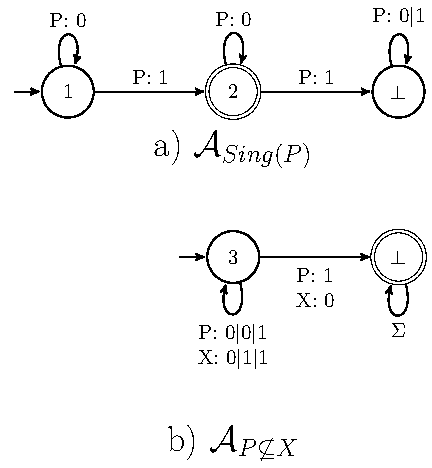
\includegraphics{fig/formula-singleton-and-subset.pdf}}
  \scalebox{0.7}{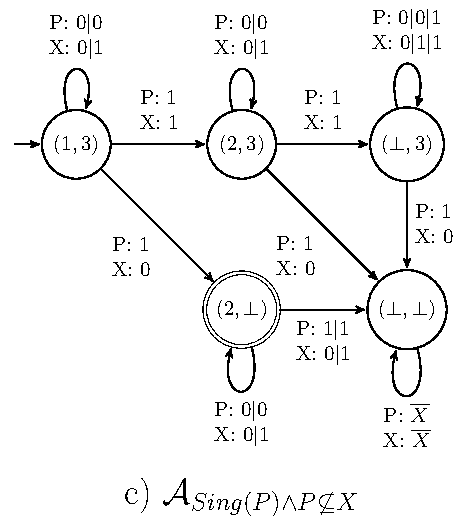
\includegraphics{fig/formula-automaton-product.pdf}}
  \scalebox{0.7}{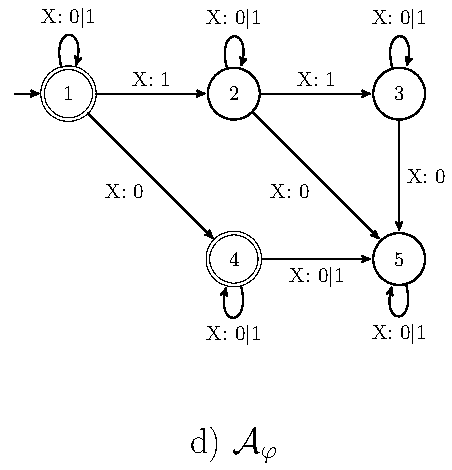
\includegraphics{fig/formula-automaton.pdf}}
 \end{center}
 \caption{Finite automata corresponding to all the subformulae of the given
 formula $\rho \overset{\mathit{def}}{=} \exists P:
 Sing(P) \wedge P \not\subseteq X$}\label{automata}
\end{figure}
   \noindent\hrulefill
   
In implementation terms existential quantification is therefore equivalent to
the operation of a~projection on the automaton. This raises an issue with
final states of the constructed automaton $\mathcal{A}$, since the projection
erases some of the transition tracks of the automaton and thus may introduce
non-determinism. Such an automaton has to be determinised, yielding DTA
$\mathcal{A}'$.

However, the automaton $\mathcal{A}'$ is not enough, since searched witness of
some model can be longer after the operation of projection. $\mathcal{A}'$ needs
to be further modified to correctly represent encodings of all models of
formula.
Consider e.g. the assigment $X \mapsto \{111\}, Y \mapsto \{11\}$, encoded as
$(\substack{X:
001\\Y: 010})$, as being a model of formula $\psi$. When we perform projection
on~$X$ over the model, the resulting encoding $(Y: 010)$ is not a valid encoding of
the model $Y \mapsto \{11\}$, which would be $(Y: 01)$.

\begin{defz}
We define the~\emph{right-quotient} of a~language $L$ with a~language $L'$ as:
\begin{equation}
 L / L' = \{w \mid \exists u \in L' : w\cdot u \in L\}.
\end{equation}
\end{defz}

\noindent Now we define the language $L^i$ as
\begin{equation}
 L^i = \{w \in \{\{0, 1\}^k\}^* \mid \text{the $j$-th track of word } \mathit{w}
 \text{ is of the form $0^*$ for $j \neq i$}\}. \end{equation}
 
 The language of the automaton $\mathcal{A}'$ after projection $\gamma_i$ on
 the $i$-th track is then defined as
 \begin{equation}
  L(\mathcal{A}') = \gamma_i(L(\mathcal{A}) / L^i).
 \end{equation}
 
 In \textsc{MONA}~\cite{mona} this is done in $\mathcal{O}(n)$ time by using
 the breadth-first search by backwards exploration of the automaton from final
 states followed by the subset construction of the determinised automaton
 yielding only reachable states.

\begin{prop}
 Since there is a~\emph{one-to-one} correspondence between models of $\phi$ and
 trees accepted by $\mathcal{A}_\phi$, $\phi$ is satisfiable iff
 $L(\mathcal{A}_\phi)$ is non-empty and valid iff $L(\mathcal{A}_\phi)$  is
 universal.
\end{prop}

The computational complexity of WS$k$S is in the NONELEMENTARY
class~\cite{wsksisnonelementary}, so given a Turing machine $\mathcal{M}$ deciding a~satisfiability of WS$k$S formulae, for
any $u \geq 0$, there are infinitely many $n$ for which a~computation of
$\mathcal{M}$ for some sentence of length $n$ requires at least
$$\underbrace{2^{2^{\iddots^{2^n}}}}_u$$ steps.
	
\chapter{\textsc{MONA}}\label{monachap}

 \textsc{MONA}~\cite{mona} is one of the early implementations of a~decision
 procedure for the WS$k$S logic, namely for $k = 1$ and $k = 2$ (note that it
 can be shown that an arbitrary $k$ can be transformed into formula in WS2S).
 WS1S can be used for a description of linear structures like linked lists or
 chains, while WS2S is mainly used for binary tree structures like a binary tree
 or a binary heap. After many years it is still the best and fastest approach
 for deciding WS$k$S formulae with the use of deterministic automata. It is an
 implementation of the decision procedure from Chapter \ref{classical} with a~few tweaks that we
 describe in this chapter.

The development of \textsc{MONA} started in 1984 and in the following years
numerous approaches were tried out and a number of fine optimizations were discovered.
In this chapter we review some of the design choices and implementation tricks
that stand behind its success.

\section{The main issue of the use of deterministic tree automata}

Considering a WS$k$S formula with a~fixed number of quantifier alternations $N$,
the decision method outlined in the previous section works in the time which is
a tower of exponentials with the height being $O(N)$.

This is mainly because every time we encounter a~sequence of quantifiers, we
have to do a~projection, which yields a~non-deterministic automaton, even if the
input automaton was deterministic. When we encounter a~negation of a
formula, we have to use determinization in order to complement the automaton,
which requires in general an exponential time and the space w.r.t the number of
states of the automaton.

Therefore every time non-determinism is introduced to the automaton, the
automaton is determinised and the information about the original states is
forgotten. So the \textsc{MONA} approach has issues with extensive the use of
an automaton complementation and since there is no known tree automaton
complementation technique better than bottom-up determinization of the automaton
followed by swapping final and non-final states, \textsc{MONA} had to come up
with heavy optimizations and heuristics to achieve good results.
\newpage
 \section{The used optimizations}\label{monasecrets}
\subsection{Using BDDs for automata representation}\label{monabdd}
BDDs were introduced to solve problems of large input alphabets, which also
allowed numerous specialized algorithms to be used.

BDDs were described in Section \ref{bdd}; they are useful for its compactness,
canonicity and efficient manipulation. \textsc{MONA} uses shared MTBDDs with
roots and leaves representing states of an automaton. The use of BDDs for
representation of transition relation proved to have the highest effect on the
formulae that could not be decided in a~fixed limit of time that was set up during benchmarks.

\subsection{Caching}
The implementation of the BDDs, as stated in Section \ref{monabdd}, is optimized
to minimize the number of cache misses that occur, since it was discovered that
cache misses dominate the running time for both the unary and binary BDD apply
operations on a 296\,MHz UltraSPARC CPU with 1\,GB
RAM.

Nodes are thus stored directly under the hash address to minimize the 
number of cache misses, as opposed to the traditional approach that stores nodes
separately from the hash table containing pointers to them, which roughly doubles the time to
access a~node.

\subsection{Eager minimization}
Whenever MONA performs the product or projection operation during the
translation from a formula to an automaton, the Myhill-Nerode minimization takes
place, since it is preferable to operate with as small automata as possible.
However, this approach was shown to be excessive, since the minimization
procedure often exceeds half of the total running time.

Alternatives were introduced\,---\,using one final minimization, minimizing only
after projection or minimizing only after product, which had different effects
and were dependent on particular benchmarks.

\subsection{Guided tree automata}

The set of states is partitioned in order to split a~large tree automaton into
several smaller ones to address expensive computations caused by
three-dimensional transition tables. This however requires for user to specify the \emph{guide}
which is a~top-down deterministic tree automaton that assigns state spaces to
the nodes of a~tree.

\subsection{Directed Acyclic Graph representation}\label{dag}

The frontend of the MONA tool is parsing the input files with specification of
WS$k$S formulae. This file is converted to the inner representation of
automata-theoretic operations, that are further translated to the resulting
automaton.

There are, however, many common subformulae with a similar structure, especially
if we talk about \emph{signature equivalence}, which holds for two formulae $\phi$
and $\psi$ if there is an order-preserving renaming of the variables in formulae
such that the representations of $\phi$ and $\psi$ become identical.

It holds for the BDD representation that automata for signature-equivalent trees
are isomorphic in the sense that only node labels differ, which means these
representations can be reused simply by renaming variable nodes. Thus MONA
represents input formulae in the form of \emph{directed acyclic graph} and not a
tree.
\newpage
\subsection{Three-valued logic and automata}
Since formulae are translated to the restricted syntax that uses only
second-order variables, first-order variables are encoded as singletons. This
however raises the issue of \emph{restrictions}, i.e. a formula $\phi$ holds
only when some external associated restrictions hold. Since a restriction is
also a formula, the main issue is that $\phi$ is now undefined outside the
restriction. Note that for a~first-order variable, the restriction is that it is
a singleton set.

The nature of these problems are solved by using a~three-valued logic. So for a
restricted subformula $\phi$ we associate a~restriction $\phi_R$. And if for
some valuation $\phi_R$ does not hold, then the formulae containing $\phi$ are
assigned the third value \emph{don't-care}.

A~special operation converts the rejecting states to don't-cares for the
restriction formulae and other automaton operations are modified so these
nonacceptance of restrictions are propagated properly.

\subsection{Formula reductions}
Various optimizations of formulae takes place in the DAG specified in Section
\ref{dag} before the final translation to the automaton. Reductions are based on
the syntactic analysis that tries to identify valid subformulae and equivalences
among them.

MONA performs few kinds of reductions:
\begin{enumerate}
 \item Simple equality and Boolean reductions that can be described by simple
 rewrite rules like $\phi \wedge \phi \mapsto \phi$, etc. These rewrite
 steps guarantee a~reduction of complexity, but will not cause significant
 improvements in the running time, since they rarely apply in realistic
 situations. However, they are cheap and may yield small improvements.

\item Special quantifier reductions. The basic idea is to apply a~rewrite step
which removes quantifiers where they are not useful, as following:
\begin{equation}\exists X . \phi \mapsto \phi[T/X]
\end{equation}
provided that $\phi \Rightarrow X = T$ is valid formula and the term $T$ is
satisfying the constraint that $\mathit{freeVars}(T)~\subseteq~\mathit{freeVars}(\phi)$, where
$\mathit{freeVars}(T)$ denotes the set of free variables in some subformula $T$.
This is further restricted to a different rewrite rule: \begin{equation} \exists
X_i .\phi \mapsto \phi[X_j/X_i]
\end{equation} provided that $\phi \equiv
\ldots \wedge X_i = X_j \wedge \ldots$ and $X_j$ is some variable other than
$X_i$. This, however, is not guaranteed to yield better results.
\end{enumerate}

 \chapter{Deciding WS$k$S with Non-deterministic Automata}\label{our}

The \textsc{MONA} tool implementation of the decision procedure for WS$k$S from
Section \ref{classical} uses deterministic bottom-up tree automata (as described
in Chapter \ref{monachap}) and so every time non-determinism might be
introduced, such as through the union and the projection corresponding to
the disjunction and the existential quantification respectively, the automaton
is determinised using the subset construction and the information about the original states is forgotten.

While this approach makes automaton complementation easy (since
a complete deterministic automaton require only swapping final with non-final
states), the extensive determinisation is still a~serious drawback. The \textsc{MONA} tool is
thus heavily optimized for the use of deterministic finite (tree)
automata, as we introduced in Section \ref{monasecrets}. However, a~decision
procedure that uses non-deterministic automata needs to deal with the issue of
complementation, for which there is currently no known algorithm that avoids
determinisation and the respective state explosion.

In practice, the representation of all models of $\phi$ is not always necessary
and any model or an invalid assignment to free variables suffices, therefore
constructing the full automaton $\mathcal{A}_{\phi}$ representing all models of
$\phi$ can be avoided.

Current trends in formal verification and theory of automata tend to use
non-deter\-ministic automata instead of deterministic ones. This is due to the
fact that there exist optimized libraries for their use, like VATA~\cite{vata},
and recently new algorithms that are efficient in practice were developed even
for time complex operations like language inclusion or universality testing,
which are PSPACE-complete for finite word automata and EXPTIME-complete for tree
automata.

Here we propose to use an algorithm based on the principle of
antichains~\cite{tacas}, defined in the following sections, and search for an
accepting or a non-accepting state \emph{on-the-fly} without constructing the
automaton corresponding to the given formula in the first place.

\section{Antichain-based universality testing of NFAs}

We will give a~brief introduction to the universality testing for
non-deterministic finite word automata by an algorithm that uses a~combination
of the simulation-based and the antichain-based approaches~\cite{tacas}.

\newpage
\noindent\hrulefill
\begin{example}
Consider testing the validity of the formula $\rho$ from Example
\ref{wsks-formula-automaton}:
  \begin{equation}
  \rho \overset{\mathit{def}}{=} \exists P:
 Sing(P) \wedge P \not\subseteq X.
  \end{equation}
  
Given the automaton $\mathcal{A}_\rho$ corresponding to the formula $\rho$
(see Section \ref{classical}), testing validity of $\rho$ is
equivalent to testing universality of the language $L(\mathcal{A}_\rho)$, which
can be done by searching for an accepting state in the complemented automaton.

\begin{figure}[h!]
 \begin{center}
  \scalebox{0.5}{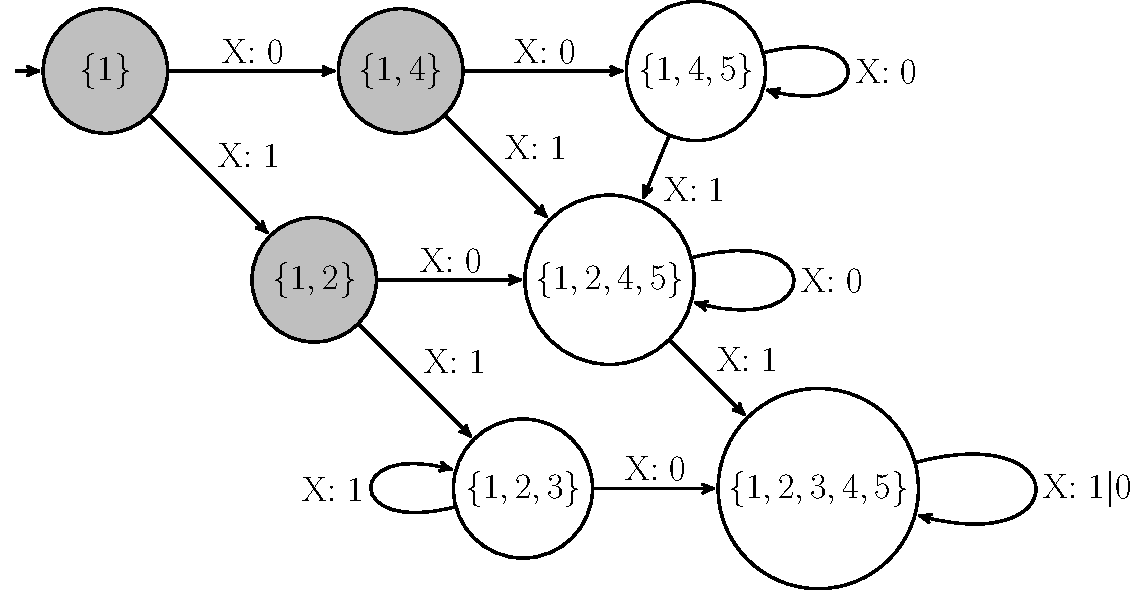
\includegraphics{fig/antichain-meets-projection.pdf}}
 \end{center}
 \caption{Comparison of the antichain-based (grey nodes) and the classical (all
 nodes) approach to universality checking.}
 \label{compare}
\end{figure}

When using the textbook approach for testing universality (by using the subset
construction and complementation), 7 states are generated as depicted in Figure
\ref{compare} If we use the antichain-based approach, then macro-states $\{1,
2\}$ and $\{1, 4\}$ are simulated by the initial state $\{1\}$ so we can
discard these states.
Since we have not reached an accepting state, we can conclude that the
language of the complemented automaton $\mathcal{A}_{\neg\rho}$ is empty, then
$\mathcal{A}_\rho$ is universal and $\rho$ is thus valid.
\end{example}
\noindent\hrulefill

\begin{defz}
A~\emph{simulation} on a~finite automaton $\mathcal{A} = (Q, \Sigma, \delta, I,
F)$ is a~relation $\preceq~\subseteq~Q \times Q$ such that $p \preceq r$
implies the following two conditions (i) $p \in F \Rightarrow r \in F$ and (ii) for
every transition $p \overset{a}{\longrightarrow} p'$, there exists a~transition $r
\overset{a}{\longrightarrow} r'$ such that $p' \preceq r'$.
\end{defz}

 We use $A^{\subseteq}$ to denote the set of relations over the states of
$\mathcal{A}$ that imply language inclusion, that is for all $\leqq \in
A^{\subseteq}$ it holds that $p \leqq r \Rightarrow L(p) \subseteq L(r)$.
Analogously we define the set of relations over the macro-states $\mathcal{A}$
that imply language inclusion as $\mathcal{A}^\sqsubseteq$.

\begin{lemma}
Given a~simulation $\preceq$ on a~NFA $\mathcal{A}$, it holds that $\preceq \in
\mathcal{A}^\subseteq$.
\end{lemma}

\begin{proof}
A proof can be found in~\cite{tacas}.
\end{proof}

The universality problem for a~NFA $\mathcal{A} = (Q, \Sigma, \delta, I, F)$ is
to decide whether $L(\mathcal{A}) = \Sigma^*$. This problem is hard, it actually
is PSPACE-complete, however, the heuristic described in~the~following works
well for many real-world examples.

The naive algorithm performs determinization using the subset construction to
obtain the~deterministic automaton $\mathcal{A}_D$, then complements it to
obtain $\overline{\mathcal{A}_D}$ and finally checks that there is no reachable
accepting state in $\overline{\mathcal{A}_D}$ (in case there is, the language
is not universal).

The algorithm proposed in~\cite{tacas} runs the subset construction procedure
\emph{on-the-fly}, avoiding explicit construction of $\overline{\mathcal{A}_D}$,
and checks if any accepting macro-state is reachable. This procedure is
further augmented with the following two optimizations.
\newpage
The first optimization is based on the following lemma.

\begin{lemma}\label{lemma2}
 Let $P, R$ be two macro-states of a~NFA $\mathcal{A}$, and $\preceq$ be a
 relation from $\mathcal{A}^\subseteq$. Then, $P \preceq^{\forall\exists} R$
 implies $L_\mathcal{A}(P) \subseteq L_\mathcal{A}(R)$, where $P
 \preceq^{\forall\exists} R$ stands for $\forall p \in P. \exists r\in R : p
 \preceq r$.
\end{lemma}

The relation $\preceq$ can be any relation on the states of $\mathcal{A}$ that
implies language inclusion, e.g. the maximum simulation or the identity
relation. When two states $P$ and $R$ such that $P \preceq^{\forall\exists}
R$ are encountered during the search for a non-accepting state, we can
discard $R$, because $L(P) \subseteq L(R)$ so $P$ has a higher chance to find
a non-accepting state. The other optimization is based on the observation that
$L_\mathcal{A}(P) = L_\mathcal{A}(P \setminus \{p_1\})$ if there is some $p_2 \in P \setminus \{p_1\}$ such that $p_1 \preceq p_2$, which is also a~simple consequence of Lemma \ref{lemma2}.

\begin{algorithm}[ht!]
		\SetKwFor{For}{foreach}{do}{}
		\SetKwRepeat{Repeat}{repeat}{until}
		\KwIn{A macro-state $I$ of an automaton $\mathcal{A}$, a~relation
		$\leqq \in A^{\sqsubseteq}$ on the macro-states of
		$\mathcal{A}$, a~successor function $\delta$ and a~predicate
		\texttt{IsFinal(F)} that decides whether a~macro-state $F$ is final}
		\KwOut{\textsc{TRUE} iff there exists a~final state in
		$\mathcal{A}$ reachable from $I$,
		\textsc{FALSE} otherwise}
		\BlankLine
				\SetKwProg{myproc}{Function}{}{}
		\BlankLine
  \myproc{\upshape \texttt{IsFinalReachable}(\textbf{state} $I$,
  \textbf{relation} $\leqq$, \textbf{post} $\delta$, \textbf{pred}
  \texttt{IsFinal})}{ \nl\uIf{{\upshape \texttt{IsFinal}}(I)}{
    	\nl\Return \textsc{TRUE}\;}
		\nl $\mathit{Processed} := \emptyset$\;
		\nl $\mathit{Next} := \{I\}$\;
		\nl\While{$\mathit{Next} \neq \emptyset$}{
		  \nl Pick and remove a~macro-state $R$ from $\mathit{Next}$ and move it to
		  $\mathit{Processed}$\;
			 \nl \uIf{{\upshape \texttt{IsFinal}}(R)}{\nl \Return \textsc{TRUE}\;}
			\nl \For{$P \in \delta(R)$}{
			 \nl \uIf{$\neg\exists S \in \mathit{Processed} \cup \mathit{Next}$ s.t. $P \leqq S$}{
			  \nl Remove all $S$ from $\mathit{Processed} \cup \mathit{Next}$ s.t. $S \leqq P$\;
				\nl Add $P$ to $\mathit{Next}$\;
			 }
			}
		}
		\nl \Return \textsc{FALSE}\;
		}
		\caption{Checking reachability of a~final state using optimized
		algorithm~\cite{tacas}}\label{universality}
	\end{algorithm}
	
The algorithm for testing universality of NFA is based on
Algorithm~\ref{universality}, which works as follows.
While there are macro-states to be processed, and no accepting macro-state has
been found, one of the macro-states from $\mathit{Next}$ is chosen and moved to
the $\mathit{Processed}$ set. All successors of the macro-state are generated,
minimized and moved to $\mathit{Next}$ unless there is already some
$\leqq$-bigger macro-state in $\mathit{Next}$ or in $\mathit{Processed}$. If
a new macro-state is added to $\mathit{Next}$, then all $\leqq$-smaller states
are pruned out of both $\mathit{Next}$ and $\mathit{Processed}$.

Testing universality of an automaton $\mathcal{A}$ is thus equivalent to
the searching for an accepting state in the automaton $\overline{\mathcal{A}_D}$
obtained by determinization and complementation of the set of final states.
	
\begin{lemma}\label{search-is-correct}
 Given the automaton $\mathcal{A} = (Q, \Sigma, \delta, I, F)$, the function
 \texttt{IsFinalReachable}($\{q\}$, $\leqq \in \mathcal{A}^\sqsubseteq$,
 $(\lambda R.\ \{\{s\} \mid \exists r \in R:\, r \overset{a}{\rightarrow} s
 \in \delta\})$, ($\lambda\ R.
 R \cap F \neq \emptyset$)) from Algorithm \ref{universality} returns
 \textsc{TRUE} iff there is a~reachable final state from state $q$ in $\mathcal{A}$.
\end{lemma}
\begin{proof}
 A proof can be found in~\cite{raskin}.
\end{proof}

\begin{lemma}\label{simulation-in-ca}
The relation $\subseteq^{-1}$ is a~simulation on the complemented automaton
$\overline{\mathcal{A}_D}$.
\end{lemma}
\begin{proof}
 A proof can be found in~\cite{raskin}
\end{proof}

\begin{lemma}
The language of an automaton $\mathcal{A} = (Q, \Sigma, \delta, I, F)$ is
universal iff the function from
Algorithm~\ref{universality} \texttt{IsFinalReachable}($I$, $\leqq \in \mathcal{A}^\sqsubseteq$,
 $(\lambda R.\ \{\{s\} \mid \exists r \in R:\, r \overset{a}{\longrightarrow} s
 \in \delta\})$, ($\lambda\ R.
 R \cap F \neq \emptyset$)) returns
\textsc{TRUE}.
\end{lemma}

\section{Deciding WS1S with NFAs}

In this section we will describe the proposed decision procedure on the simpler
case for $k = 1$, i.e. WS1S. In the next section, we will extend the procedure
to an arbitrary $k$.

Given a~formula $\phi$, the construction of the automaton $\mathcal{A}_\phi$
representing all models of $\phi$ is not always necessary and in many
applications any model or an invalid assignment suffices.
Therefore we can exploit the antichain-based techniques defined in the previous
section and search for an accepting or a non-accepting state \emph{on-the-fly}
while pruning the search space.

First, the formula $\phi$ is transformed to a~logically equivalent formula
$\varphi$ in the existential prenex form (see Section \ref{restricted}):
\begin{equation*}
 \varphi \overset{\mathit{def}}{=}
 \exists\mathcal{X}_{m+1}\neg\mathcal{X}_m\neg\ldots\neg\exists\mathcal{X}_2\neg\exists\mathcal{X}_1
 :
 \pi.
\end{equation*}

Supposing there are $m$	negations in the prefix of the formula $\varphi$, we
create a~hierarchical family of WS$k$S formulae $\Phi = \{\varphi_0,\ldots,\varphi_m\}$
where
\begin{equation}
  \varphi_0 \overset{\mathit{def}}{=} \pi
\end{equation}
and for all $0 \leq i \leq m \minus 1$
\begin{equation}
 \varphi_{i+1} \overset{\mathit{def}}{=} \neg\exists\mathcal{X}_{i+1}:\ 
 \varphi_i.
\end{equation}
The relation between this family of formulae $\Phi$ and the formula $\varphi$ is
depicted as follows:
\begin{equation}
\begin{aligned}
\varphi \overset{\mathit{def}}{=} \exists \mathcal{X}_{m+1}\,
\underset{\varphi_m}{\underbrace{
  \neg\,\exists \mathcal{X}_m\,
  \neg
  \underset{\hspace{-3mm}\iddots}{
    \dots 
    \underset{\varphi_2}{\underbrace{
      \neg \,\exists \mathcal{X}_2\,
      \underset{\varphi_1}{\underbrace{
        \neg \,\exists \mathcal{X}_1\,:\,
        \underset{\varphi_0}{\underbrace{
          \pi
        }}
      }}
    }}
  }
}}
\end{aligned}
\end{equation}

We will use the notation $\Gamma(G)$ to denote the alphabet defined as the
set of functions $\Gamma(G) = \{f : G \rightarrow \{0, 1, \bot\}\}$, with the
special case for $G = \emptyset$ defined as $\Gamma(\emptyset) = \{\#\}$. Elements of this set can
be viewed as strings of a~fixed length $|G|$ over the alphabet $\{0, 1, \bot\}$
where each position in the strings is associated with exactly one element of G.

Given the symbol $f \in \Gamma(G)$ and a~set $H \subseteq G$, the
\emph{projection} of $f$ over the set $H$, written as $\omega_H(f)$, can be
defined as the restriction of the function $f$ over the set $G\setminus H$, i.e.
$\omega_H(f) = f|_{G\setminus H}$. This can be further extended to sets of symbols. Given a
set $E \subseteq \Gamma(G)$, we define the projection over a~set $H \subseteq
G$, written $\omega_H(E)$, as $\omega_H(E) = \{\omega_H(f) \mid f \in E\}$. For
a string $w = a_1\ldots a_n \in \Gamma(G)^*$ we define the operation as
$\omega_H(w) = \omega_H(a_1)\ldots\omega_H(a_n)$.

For a~language $L \subseteq \Gamma(G)^*$, the projection of $L$ over $H$,
written as $\omega_H(L)$, is defined as $\omega_H(L) = \{\omega_H(f) \mid f \in
L\}$. Note that $\omega_H(L) \subseteq \Gamma(G\setminus H)^*$.

\begin{lemma} Given the alphabet $\Gamma(G)$, $H \subseteq G$ and $X, Y
\subseteq \Gamma(G)^*$ it holds that
\begin{equation}
 X \subseteq Y \Longrightarrow \omega_H(X) \subseteq \omega_H(Y).
\end{equation}
\end{lemma}
\begin{proof}
For each symbol $z \in \omega_H(X)$ there must exist some $x \in X$ such that
$z = \omega_H(x)$. Since $X \subseteq Y$ it must also hold that $x \in Y$, and
hence it holds that $\omega_H(x) \in \omega_H(Y)$. Therefore $\omega_H(X)
\subseteq \omega_H(Y)$.
\end{proof}

As we described in Section \ref{wsks}, there is an issue with the encoding of
all models of formula and using the projection operation on the automaton. If
the projection were implemented by only removing parts of symbols corresponding to the
variables in the existential quantification, the resulting automaton
would not accept some of the valid models of the formula,
as described by Example \ref{models}. \textsc{MONA} (see Section
\ref{classical}) solves this by adjusting the final states of the automaton by
using the breadth-first search algorithm in the linear time after every
projection of an automaton.

Note that in the following we will use the symbol $\overline{0}$ as the
substitute for the symbol $0^k$ for some known $k$.
\newpage
\noindent\hrulefill
\begin{example}
 Consider the formula $P \not\subseteq X$ and its corresponding automaton
 $\mathcal{A}_{P \not\subseteq X}$ depicted in Figure \ref{projection} with
 one final state.
 After restricting the tracks of the automaton by removing the variable $P$ we
 get the automaton $\mathcal{A}_{\exists P: P \not\subseteq X}b$ in Figure
 \ref{projection}b.
 
 After the restriction the automaton does not accept e.g. the following word
 $111$, $111 \notin L(\mathcal{A}_{\exists P: P \not\subseteq X})$, even though $X = \{1, 2,
 3\} \models \exists P: P \not\subseteq X$. However, it does accept another
 encoding of this set namely $1110 \in L(\mathcal{A}_{\exists P: P \not\subseteq
 X})$, which is not a~correct encoding according to the rules set in Chapter
 \ref{wsks}. Hence we must adjust the final states by extending it by the states
 that can reach them with words $\overline{0}^*$.
 \begin{figure}[h!]
  \begin{center}
   \scalebox{0.75}{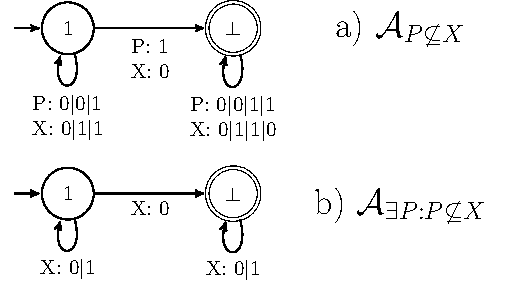
\includegraphics{fig/projection-problem}}
  \end{center}
  \caption{The issue with final states after projection is that
  the language of the resulting automaton restricts encodings
  of some valid models afterwards.}\label{projection}\label{models}
 \end{figure}\end{example}\noindent\hrulefill

Adjusting the final states needs a~fully constructed automaton, so this cannot
be used in an on-the-fly algorithm. Instead, we can either precompute the set of
final states inspired by backwards universality
testing~\cite{backwards-universality} or use a~lazy approach that will determine
whether a~state is final only when this information is actually needed.

\begin{defz}
For a~set of states $R$ of the automaton $\mathcal{A} = (Q, \Sigma, \delta, I,
F)$ we define the \emph{set of direct predecessors through zero tracks} as the
set $\mathit{PRE}_0(R)$ of states such that
\begin{equation}
 \mathit{PRE}_0(R) = \{q \in Q \mid \exists r \in R: q
 \overset{\overline{0}}{\longrightarrow} r \in \delta\}.
\end{equation}
We denote the reflexive transitive closure of $\mathit{PRE}_0(Q)$ as
$\mathit{PRE}_0^*(Q)$.
Note that we can define the $\mathit{POST}_0$ function similarly to
$\mathit{PRE}_0$.
\end{defz}

\begin{defz}
 Given the automaton $\mathcal{A} = (Q, \Sigma, \delta, I, F)$ we define the
 \emph{projection} $\omega_\mathcal{X}$ of $\mathcal{A}$ over the set of
 variables $\mathcal{X}$ as the automaton $\omega_\mathcal{X}(\mathcal{A}) = (Q,
 \omega_{\mathcal{X}}(\Sigma), \omega_{\mathcal{X}}(\delta), I,
 \mathit{PRE}_0^*(F))$ where
 \begin{equation}
  \omega_{\mathcal{X}}(\delta) = \left\{ p \overset{\omega(a)}{\longrightarrow}
  r \mid p \overset{a}{\longrightarrow} r \in \delta\right\}.
 \end{equation}
 Note that the result of projection has the final states adjusted
 according to the $\mathit{PRE}_0$ relation.
\end{defz}

\begin{defz}
 Given the automaton $\mathcal{A} = (Q, \Sigma, \delta, I, F)$ we define the
 \emph{complementation} $\gamma$ of $\mathcal{A}$ as the automaton
 $\gamma(\mathcal{A}) = (2^Q, \Sigma, \delta_\gamma, \{I\}, \{S \subseteq Q\
 |\ S \cap F = \emptyset\})$ where
 \begin{equation}
  \delta_\gamma = \{R \overset{a}{\longrightarrow} S \mid S = \{s \in Q \mid \exists
  r \in R: r \overset{a}{\longrightarrow} s \in \delta\}\}.
 \end{equation}
 Note that this operation $\gamma$ corresponds to the determinisation of the
 input automaton using the subset construction followed by swapping final and
 non-final states of the determinised automaton.
\end{defz}

Given a~WS$1$S formula $\varphi$ in the $\exists$PNF form, the automaton for
the matrix $\pi$ of the formula, $\mathcal{A}_\pi$, can be constructed out of
the automata corresponding to the atomic formulae and their complements by
using the operations of union and intersection only (see Section
\ref{classical}).
Further, $\mathcal{A}_\varphi$ could be constructed from the automaton $\mathcal{A}_\pi$ by successive
applications of complementation~$\gamma$ and projection~$\omega$ according to
the prefix of $\varphi$ as these operations were defined before. But we take a~different path.

% \begin{defz}
%  We define the \emph{downward closure} of a~set $S$ as set $\downarrow S$ such
%  that
%  \begin{equation}
%   \downarrow S \overset{\mathit{def}}{=} \{p\in Q \mid \exists q \in S: p
%   \subseteq q\}
%  \end{equation}
% \end{defz}
% 
% \begin{defz}
%  Similarly we define the \emph{upward closure} of a~set $S$ as set $\uparrow S$
%  such that
%  \begin{equation}
%  \uparrow S \overset{\mathit{def}}{=} \{p\in Q \mid \exists q \in S: q \subseteq
%  p\}
%  \end{equation}
% \end{defz}

% \begin{defz}
%  We define the \emph{preset through zero tracks} as a~set of states such that
%  \begin{equation}
%  PRE_0(Q) = \{r \mid \exists q \in Q: r \overset{(0)^k}{\longrightarrow}
%  q\}.\footnote{Note that $(0)^k$ does stand for zero track of width $k$ not
%  length.}
%  \end{equation}
%  We denote the transition closure of $PRE_0(Q)$ as $PRE_0^*(Q)$. Note that we
%  can define the $POST_0(Q)$ relation simiralry to the $PRE_0$ relation.
% \end{defz}

Analogously to the family of formulae $\Phi$, we can define
the family of automata $\mathbb{A} = \{\mathcal{A}_0,\ldots,\mathcal{A}_m\}$ as follows:
 \begin{eqnarray}
  \mathcal{A}_0 & = & \mathcal{A}_\pi,\\
  \mathcal{A}_{i+1} & = & \gamma(\omega_{\mathcal{X}_{i+1}}(\mathcal{A}_i)).
 \end{eqnarray}
 
 Note that the automaton $\mathcal{A}_i$ then corresponds to the following
formula:
 \begin{equation} \varphi_i =
 \neg\exists\mathcal{X}_i\ldots\neg\exists\mathcal{X}_1.
 \pi.
 \end{equation}
 
 We use the notation $\mathcal{A}_i = (Q_i, \Sigma_i, \delta_i, I_i, F_i)$ to
 address a~particular automaton and its components.
There is a~further connection between the hierarchical family of formulae $\Phi$
and the hierarchical family of automata $\mathbb{A}$ as described by the
following lemma.
 \begin{lemma}\label{uni-valid} For all $0 \leq i \leq m$, the language of
$\mathcal{A}_i$ is
\begin{enumerate}
  \item \emph{universal} iff $\varphi_i$ is \emph{valid},
  \item \emph{non-empty} iff $\varphi_i$ is \emph{satisfiable},
  \item \emph{non-universal} iff $\varphi_i$ is \emph{invalid}, and
  \item \emph{empty} iff $\varphi_i$ is \emph{unsatisfiable}.
\end{enumerate}
\end{lemma}

\begin{proof}
A proof of this Lemma can be found in~\cite{tata}.
%  This can be proved by induction on $i$. With base case $i = 0$ holding due to a
%  proposition \ref{prop}. We can further prove this lema for case $i = n + 1$
%  supposing it holds for some $n$, i.e. the language of $\mathcal{A}_n$ is
%  \begin{enumerate}
%    \item universal iff $\varphi_n$ is valid,
%    \item non-empty iff $\varphi_n$ is satisfiable,
%    \item non-universal iff $\varphi_n$ is invalid, and
%    \item empty iff $\varphi_n$ is unsatisfiable.
%  \end{enumerate}
%  
%  We define the formula $\varphi_{n+1}$ as 
%  \begin{equation}
%  \varphi_{n+1} \overset{\mathit{def}}{=} \neg\exists\mathcal{X}_{n+1}.
%  \varphi_n.
%  \end{equation}
%  
%  Now we will consult each of the cases of the validity, or satisfiablity, of
%  given formula $\varphi_n$:
%  \begin{enumerate}
%    \item Suppose that $\varphi_n$ is valid. Then after the projection over set
%    of variables $\mathcal{X}_{n+1}$ the formula is still valid and the negation
%    of the formula $\varphi_{n+1} = \neg\exists\mathcal{X}_{n+1}.\varphi_n$ is
%    thus unsatisfiable. By the induction hypothesis it holds, that the language
%    $L(\mathcal{A}_n)$ is universal. After projection the language
%    $\omega_{\mathcal{X}_{n+1}}(L(\mathcal{A}))$ is also universal and the
%    negation thus makes the language $L(\mathcal{A}_{n+1})$ empty.
%    \item Suppose that $\varphi_n$ is satisfiable. Then after projection formula
%    $\exists\mathcal{X}_{n+1}. \varphi_n$ is also satisfiable (since, the
%    projection yields bigger or equivalent language) and the negation of the
%    formula $\varphi_{n+1} = \neg\exists\mathcal{X}_{n+1}.\varphi$ is thus
%    invalid. From induction hypotesis it holds that the language
%    $L(\mathcal{A}_n)$ is non-empty. After the projection the language remains
%    non-empty and so the negation of the formula yields non-universal language
%    $L(\mathcal{A}_{n+1})$.
%    \item Suppose that $\varphi_n$ is unsatisfiable. Then after projection
%    formula $\exists\mathcal{X}_{n+1}$ is still unsatisfiable, which means that
%    the negation of the formula $\neg\exists\mathcal{X}_{n+1}$ is valid. By
%    induction hypothesis the language $L(\mathcal{A}_n)$ is empty. The projection
%    of the language $\omega_{\mathcal{X}_{n+1}}(L(\mathcal{A}_n))$ is still empty
%    and so the negation of the formula yields univesal language.
%    \item Suppose that $\varphi_n$ is invalid. Then after projection formula
%    $\exists\mathcal{X}_{n+1}$ can either be still invalid or can become valid,
%    after the augmentation of the final states. Thus we have to distinguish two
%    cases:
%    \begin{enumerate}
%      \item Let us assume thet formula $\exists\mathcal{X}_{n+1}\varphi_n$ is
%      invalid.
%      Then after negation formula $\neg\exists\mathcal{X}_{n+1}\varphi_n$ is
%      satisfiable. By induction hypothesis the language $L(\mathcal{A}_n)$ is
%      non-universal. After the projection the language is still non-universal and
%      so the negation of the formula yields non-empty language.
%      \item Let us assume that formula $\exists\mathcal{X}_{n+1}\varphi_n$ is
%      valid. Then after negation formula $\neg\exists\mathcal{X}_{n+1}\varphi_n$
%      is unsatisfiable. By induction hypthesis the language $L(\mathcal{A}_n)$ is
%      non-universal. After the projection the language become universal and so
%      the negation of the formula yields empty language.
%    \end{enumerate}
%  \end{enumerate}
\end{proof}


% Further we can construct automaton $\mathcal{A}_{i+1}$ from automaton
% $\mathcal{A}_i = (Q_i, \Sigma_i, \delta_i, I_i, F_i)$ as follows:
% \begin{eqnarray}
%  Q_{i+1} & = & 2^{Q_i}\\
%  \Sigma_{i+1} & = & \Sigma_{i|\omega_{\mathcal{X}_{i+1}}}\\
%  \delta_{i+1} & = & \{P \overset{\omega_{\mathcal{X}_{i+1}}(a)}{\longrightarrow}
%  R \mid R = \bigcup_{p \in P} \{r \mid p \overset{a}{\rightarrow} q \in \delta_i\}, a~\in
%  \Sigma_i\}\\
%  I_{i+1} & = & \{I_i\}\\
%  F_{i+1} & = & \downarrow\overline{\{Q \mid Q = PRE_0^*(P), P \in F_i\}}\label{F}
% \end{eqnarray}
% 
% Notice that the set of the final states $F_{i+1}$ is computed from the states of
% the previous level of quantification. First we need to compute the predecessors
% of every final state which yields the following set
% \begin{equation}
%  F_{\exists\mathcal{X}_{i+1}\varphi_i} = \{Q \mid Q = PRE_0^*(P), P \in F_i\}
% \end{equation}
% Now to obtain the set of final states for complement of the automaton, we would
% first have to determinise the set to set
% \begin{equation}
%  F^{DET}_{\exists\mathcal{X}_{i+1}\varphi_i} = \uparrow\{ \{s\} \mid s \in
%  F_{\exists\mathcal{X}_{i+1}\varphi_i}\}
% \end{equation}
% We can complement this set and hence get the equation \ref{F}.

Given the automaton $\mathcal{A}_0$ and the sequence of sets of second-order
variables $(\mathcal{X}_1,\ldots,\mathcal{X}_m)$ corresponding to the matrix
and the prefix of $\varphi$ respectively, we can classify the formula according
to the existence of satisfying and unsatisfying assignments.

\begin{defz}
We say a~formula $\phi$ is \emph{closed} iff there is no free variable in
$\phi$, i.e.
$\mathit{freeVars}(\phi) = \emptyset$.
We further define the \emph{existential closure} of a~formula $\varphi$ as
the formula $\exists\mbox{-}\mathit{cl}$ such that
\begin{equation}
 \exists\mbox{-}\mathit{cl}(\varphi) = \exists\mathcal{X}:\ \varphi
\end{equation}
where
\begin{equation}
 \mathcal{X} = \mathit{freeVars}(\varphi).
\end{equation}

Note that we can construct an automaton corresponding to the existential closure
of a~formula $\varphi$ as $\widetilde{\mathcal{A_\varphi}} =
\omega_\mathcal{X}(\mathcal{A}_\varphi)$.
It is obvious that since the formula has no free variables, the symbols on
transitions in $\widetilde{\mathcal{A}_\varphi}$ are $\#$.
\end{defz}

\begin{lemma}\label{exists-example}
Let $\varphi$ be a~closed WS1S formula. Then $\varphi$ has a~model
iff there is an initial state of $\mathcal{A}_\varphi = (Q, \Sigma, \delta, I,
F)$ that is final, i.e.
\begin{equation}
 I_m \cap F_m \neq \emptyset \Leftrightarrow\ \models \varphi.
\end{equation}
\end{lemma}

\begin{proof}
This is implied by Lemma \ref{uni-valid}
\end{proof}

We can extend this notion to any WS1S formula $\psi$ by computing the
closure of the formula $\psi$ to yield a~formula $\varphi$ and test the validity
of the formula as stated by Lemma \ref{exists-example}.

% \begin{lemma}
% There exists a~unsatisfying assigment (counter-example) for formula $\varphi$ if
% the initial state of automaton $\widetilde{\mathcal{A}}_{\neg\varphi}$
% corresponding to the closure of formula $\varphi$ is final.
% \end{lemma}
% 
% \begin{proof}
% The proof is similar to the proof of Lemma \ref{exists-example}.
% \end{proof}
% 
% \begin{lemma}\label{example-deciding-link}
% The following lemma describes the correspondence between satisfying and
% unsatisfying examples and validity/satisfiability of formula. WS$k$S formula
% $\phi$ is
% \begin{enumerate}
%   \item \emph{unsatisfiable} iff there is no satisfiable assigment,
%   \item \emph{satisfiable} iff there exists a~satisfiable assigment,
%   \item \emph{valid} iff there is no unsatisfiable assigment.
% \end{enumerate}
% \end{lemma}
% \begin{proof}
% This comes from the definition of (in)validity and (un)satisfiability
%~\cite{sat}.
% \end{proof}

To optimize the algorithm of validity testing for WS1S formulae, we are going
to define the necessary relations so that we can prune the state space during
the search for an~accepting or a~rejecting state. 

\begin{defz}\label{simulation-definition}
 For all $0 \leq i \leq m$ we define the relation $\leq_i \subseteq Q_i \times
 Q_i$ as follows:
 \begin{eqnarray}
  \leq_0 & = & \text{id},\\
  A \leq_{i+1} B & \Leftrightarrow & \forall b \in B \exists a~\in A: a \geq_i
  b.
 \end{eqnarray}
\end{defz}

\begin{lemma}
 For all $0 \leq i \leq m$ the relation $\leq_i$ is a~simulation on
 $\mathcal{A}_i = (Q_i, \Sigma, \delta_i, I_i, F_i)$.
\end{lemma}
\begin{proof}
 We will prove this lemma by induction on the level $i$ of the relation.
 
 \begin{enumerate}
   \item The base case $i = 0$: From the definition of relation $\leq_i$,
   $\leq_0$ is equal to the identity relation, which is
   a~simulation~\cite{tacas}.
   \item Now let us take the following induction hypothesis:
 \end{enumerate}
 \begin{equation}
  \leq_n \texttt{ is a simulation on } \mathcal{A}_n.
 \end{equation}
 Further we wil prove the lemma for $n+1$, i.e. that the relation $\leq_{n+1}$
 such that
 \begin{equation}
 A \leq_{n+1} B \overset{\mathit{def}}{\Leftrightarrow} \forall b \in B
 \exists a \in A. a \geq_n b
 \end{equation}
 is a simulation.
 
 The relation $\leq_n$ is a~simulation on $\omega_{n+1}(\mathcal{A}_n)$,
 since if $a \geq_n b$ then it also holds that
 $\omega_{n+1}(a) \geq_n \omega_{n+1}(b)$.
 
 Now to prove that $A \leq_{n+1} B$ is a~simulation we need to show that the
 following formula is true for all $x \in \Sigma$:
 \begin{equation}
 (A \overset{x}{\rightarrow} A' \Rightarrow (\exists B'. B
 \overset{x}{\rightarrow} B' \wedge A' \leq_{n+1} B')) \wedge (A \in F_{n+1}
 \Rightarrow B \in F_{n+1}).
 \end{equation}
 We consider the following case split:
 
 \begin{itemize}
   \item[a)] $(A \overset{x}{\rightarrow} A' \Rightarrow (\exists B'. B
 \overset{x}{\rightarrow} B' \wedge A' \leq_{n+1} B'))$:
 \end{itemize}
 
 This condition can be further elaborated into the following formula:
 
 \begin{eqnarray}
 \begin{aligned}
  & (A \overset{x}{\rightarrow} \{a' \mid \exists a \in A. a
 \overset{x}{\rightarrow} a' \in \delta_n\}) \Rightarrow\\
  & \Rightarrow ( (B
 \overset{x}{\rightarrow} \{b' \mid \exists b \in B. b \overset{x}{\rightarrow}
 b' \in \delta_n\}) \wedge \forall b' \in B' \exists a' \in A'. a' \geq_n b')
 \end{aligned}
 \end{eqnarray}
 
 Since $A \leq_{n+1} B$, so $\forall b \in B.\ \exists a \in A.\ b \leq_n a$,
 it holds that $\forall b' \in \{b' \mid \exists b \in B. b
 \overset{x}{\rightarrow} b' \in \delta_n\}$ there is some $a' \in \{a' \mid
 \exists a \in A.\ a \overset{x}{\rightarrow} a' \in \delta_n\}$ such that $b'
 \leq_n a'$. Because, if there did not exists such $a'$, then $A \leq_n B$ could
 not be a~simulation in the first place.
 
 \begin{itemize}
   \item[b)] $A \in F_{n+1} \Rightarrow B \in F_{n+1}$:
 \end{itemize}
 A macro-state A is final on the level $i$ if it does not contain a~state on
 the level $i\minus 1$ which is final, i.e. $A \in F_{n+1}
 \overset{\mathit{def}}{\Leftrightarrow} \neg\exists a \in A.\ a \in F_n$. If
 there is no final state in $A$, then there will surely be no final state in $B$
 because $A$ has a bigger language than $B$.
 
 We have shown that both formulae of the conjuction a) and b) are true and thus
 the relation $\leq_{n+1}$ is a simulation on $\mathcal{A}_{n+1}$.
 
\end{proof}

% given automaton A0, sets {X1,..,Xm}
% 
% Fm = computeFinalStates()
% example = findSatisfyingExample()
% counter-example = findUnsatisfyingExample()
% if !example:
%   return UNSAT
% else if example & !counter-example:
%   return VALID
% else:
%   return, SAT

\begin{defz}
Given the automaton $\mathcal{A} = (Q, \Sigma, \delta, I, F)$ we define the
restriction of $\mathcal{A}$ to zero tracks as
the automaton $\mathcal{A}^0 = (Q^0, \{\overline{0}\}, \delta^0, I, PRE_0^*(F))$
where
\begin{eqnarray}
 Q^0 & = & \{q \in Q \mid \exists w \in \overline{0}^*: f
 \overset{w}{\longrightarrow} q, f \in I\},\\
 \delta^0 & = & \{p \overset{\overline{0}}{\longrightarrow} q \mid p
 \overset{\overline{0}}{\longrightarrow} q \in \delta\}.
\end{eqnarray}
\end{defz}

Note that all states are final due to the adjustment of states after projection.
The final Algorithm \ref{deciding-wsks-alg} is based on the universality
checking algorithm as described in this chapter:

\begin{algorithm}[ht!]
		\SetKwFor{For}{foreach}{do}{}
		\SetKwRepeat{Repeat}{repeat}{until}
		\KwIn{The initial state $I_m$ of the automaton $A_{\neg\varphi_m}$,
		a~relation on macro-states $\leqq \in \mathcal{A}^\sqsubseteq$}
		\KwOut{\textsc{TRUE} iff the formula $\varphi$ is valid,
		\textsc{FALSE} otherwise}
		\BlankLine
		\nl \Return \texttt{IsStateAccepting}($I_m$, $m$)
		\SetKwProg{myproc}{Function}{}{}
		\BlankLine
  \myproc{\upshape \texttt{IsStateAccepting}(\textbf{state} $P$, \textbf{level}
  $i$)}{ 
  \nl \uIf{i = 0}{
  	\nl 	\Return $P \in F_0$\;}
  	\nl \uElse{
  	\SetEndCharOfAlgoLine{}
  		\nl \For{$p \in P$}{
  			\nl \uIf{\upshape \texttt{IsFinalReachable}($p$, $\leqq$,
  			$\delta^0_{i-1}$, ($\lambda$ $q$. \texttt{IsStateAccepting}($q$, $i
  			\minus 1$)))}{ \nl \Return \textsc{FALSE}\;
  	   		}
  		}
  		\nl \Return \textsc{TRUE}\;
  	  }
  }
		\caption{Algorithm for deciding the validity of a~WS$k$S
		formula $\varphi$}\label{deciding-wsks-alg}
	\end{algorithm}

% workset = Q
% while workset != empty:
%    q = workset.pop()
%    

\section{Deciding WS$k$S}

In the previous section we introduced the concept of the algorithm for deciding
WS$1$S formulae using non-deterministic finite automata (or unary tree
automata).
We will briefly describe an extension of this procedure to an arbitrary $k$.

We extent the notion of projection to trees. Given a~tree $t :
\mathbb{N}^* \rightarrow \Gamma(G)$ the projection of $t$ over $H \subseteq G$
is defined as $\omega_H(t) = \{(n, \omega_H(f)) \mid (n, f) \in t\}$. Note that
$\omega_H(t) : \mathbb{N}^* \rightarrow \Gamma(G\setminus H)$.

Similarly to the logic WS$1$S we will define the hierarchical family of tree
automata $\mathbb{A} = \{\mathcal{A}_0,\ldots,\mathcal{A}_m\}$ where
\begin{equation}
 \mathcal{A}_0 = (Q_0, \Sigma_0, \delta_0, F_0)
\end{equation} is a~non-deterministic finite tree automaton corresponding to the
WS$k$S formula $\varphi_0 \overset{\mathit{def}}{=} \pi(\mathbb{X})$, such that
$\Sigma_0 = \Gamma(\mathbb{X})$ and
\begin{equation}
 \mathcal{A}_{i+1} = (Q_{i+1}, \Sigma_{i+1}, \delta_{i+1}, F_{i+1})
\end{equation}
is a~tree automaton corresponding to the formula $\varphi_{i+1}
\overset{\mathit{def}}{=} \neg\exists\mathcal{X}_{i+1}: \varphi_i$ where
\begin{eqnarray}
 Q_{i+1} & = & 2^{Q_i},\\
 \Sigma_{i+1} & = & \omega_{\mathcal{X}_{i+1}}(\Sigma_i),\\
 F_{i+1} & = & \{R \in Q_{i+1} \mid R \cap F_i = \emptyset\},\\
 \delta_{i+1} & = & \{(R_1,\ldots,R_t)
 \overset{\omega_{\mathcal{X}_{i+1}}(f)}{\longrightarrow} S\},
\end{eqnarray}
where
\begin{equation}
S = \{s \in Q_i \mid \exists r_1 \in R_1,\ldots,r_t \in R_t.
 (r_1,\ldots,r_t) \overset{f}{\longrightarrow}, s\}.
\end{equation}

In order to be able to talk about possible \emph{futures} of states of automata
from family of $\mathbb{A}$ we exploit the notion of languages of the so called
\emph{open trees} as defined in~\cite{tacas}.

Consider a~ranked alphabet $\Sigma$, we define a~special symbol $\square \notin
\Sigma$ with rank 0, called a~\emph{hole}. Then an \emph{open tree} over
$\Sigma$ is a~tree over $\Sigma \cup \{\square\}$ such that all its leaves are
labeled by symbol $\square$. we use $T_\Sigma^\square$ to denote the set of all
open trees over $\Sigma$. Given states $q_1,\ldots,q_n$ of the automaton
$\mathcal{A} = (Q, \Sigma, \delta, F)$ and an open tree $t$ with leaves
$v_1,\ldots,v_n$, a~run $\pi$ of $\mathcal{A}$ on $t$ from $(q_1,\ldots,q_n)$ is
defined in similar way as the run on a~tree except that for each leaf $v_i, 1
\leq i \leq n$, we have $\pi(v_i) = q_i$. We use $t(q_1,\ldots,q_n)
\overset{\pi}{\Longrightarrow} q$ to denote that $\pi$ is a~run of $\mathcal{A}$
on $t$ from $(q_1,\ldots,q_n)$ such that $\pi(\epsilon) = q$. We define the
notation $t(q_1,\ldots,q_n) \Longrightarrow q$ similarly to runs on trees.

The language of $\mathcal{A}$ accepted from a~tuple $(q_1,\ldots,q_n)$ of states
of $Q$ is $L^\square_\mathcal{A}(q_1,\ldots,q_n) = \{t \in T^\square_\Sigma
\mid t(q_1,\ldots,q_n) \Longrightarrow q \text{for some } q \in F\}$. Then
language of $\mathcal{A}$ accepted from a~tuple $(S_1,\ldots,S_n)$ of sets of
states from $\mathcal{A}$ is defined as
follows:
\begin{equation}
L_\mathcal{A}^\square(S_1,\ldots,S_n) = \bigcup_{(s_1,\ldots,s_n) \in
S_1\times\ldots\times S_n} L_\mathcal{A}^\square(s_1,\ldots,s_n).
\end{equation}

Given the vector $\overset{\rightarrow}{q_n} = (q_1,\ldots,q_n)$ of states, we
use the notation $L_\mathcal{A}^\square$ to denote the language of open trees
$L_\Sigma^\square$. Further we use the notation $\overset{\rightarrow}{q_n}[e
\mapsto s]$, where $1 \leq e \leq n$, to denote the vector
$(q_1,\ldots,q_{e-1}, s, q_{e+1},\ldots,q_n)$. This notion can be further
extended to vectors of sets of states.

Further we extent the notion of pruning states as defined in previous sections
over the languages of open trees by the following lemmas.

\begin{lemma}
Let $\sqsubseteq_i \subseteq Q_i \times Q_i$, $0 \leq i \leq m-1$, be a~relation
on the states of the automaton $\mathcal{A}_i$ such that implies inclusion of
languages of open trees, i.e.
\begin{equation}
 a \sqsubseteq_i b \Rightarrow \forall 1 \leq e \leq n. \forall
 \overset{\rightarrow}{q_n} \in Q_i^n.
 L_{\mathcal{A}_{i}}(\overset{\rightarrow}{q_n}[e \mapsto a]) \subseteq
 L_{\mathcal{A}_{i}}(\overset{\rightarrow}{q_n}[e \mapsto b])
\end{equation}
then $\forall p, r \in Q_i$, $S \subseteq Q_i$ and $\overset{\rightarrow}{V_n}
\subseteq Q^n_i$, $1 \leq e \leq n$, it holds that
\begin{equation}
 p \sqsubseteq_i r \Rightarrow
 L_{\mathcal{A}_{i+1}}(\overset{\rightarrow}{V_n}[e \mapsto (\{p, r\} \cup S)])
 \subseteq  L_{\mathcal{A}_{i+1}}(\overset{\rightarrow}{V_n}[e \mapsto (\{r\}
 \cup S)])
\end{equation}
where $(\{p, r,\} \cup S)$, $(\{r\} \cup S)$ are states of the automaton
$\mathcal{A}_{i+1}$.
\end{lemma}

\begin{proof}
Proof can be found in~\cite{tacas}.
\end{proof}

\begin{defz}
For all $0 \leq i \leq m$ we define the family of relations
$\{\sqsubseteq_i^0,\ldots,\sqsubseteq^i_i\}$ over the states of the automaton
$\mathcal{A}_i$ such that $\forall 0 \leq k \leq i: \sqsubseteq_i^k\subseteq Q_i
\times Q_i$ as follows:
\begin{eqnarray}
 \sqsubseteq_0 & = & \text{id},\\
 \sqsubseteq_i & = & \{(A, B) \mid \forall b \in B \exists a \in A. a
 \sqsupseteq b\}.
\end{eqnarray}
\end{defz}

We can use the Algorithm \ref{deciding-wsks-alg} described in previous section
to decide any WS$k$S with operation of projection extended over the trees.
Further we can use relations previously defined to prune the state space
similarly to word automata.

\chapter{Implementation}\label{impl}

As depicted in Figure \ref{flow}, the input of the implemented application is
a collection of WS$1$S or WS$2$S formulae written using the \textsc{MONA}
syntax as described in Appendix \ref{syntax}. The frontend of the
created application is reused and slightly modified parser of tool \textsc{MONA}
that is based on \texttt{yacc}~\cite{yacc} parser generator. The input file is
parsed into an intermediate representation as an Abstract Syntax
Tree (AST) with logical connectives or atomic formulae as
tree nodes. While parsing the input file, a~symbol table is filled up with the
used first or second-order variables and defined predicates or macros. 

We enhance the frontend as follows. Mapping of variables to MTBDD tracks
can be constructed in several possible ways.
Either it can correspond to the place of the definition of the variable during
the parsing process, chosen randomly or match the sequence of quantifiers from
the prefix. We prefer the last option, because projection of lower-leveled MTBDD
nodes is more efficient than higher-level nodes.

The AST is then flattened according to the rules for translation to
the restricted syntax and transformed into
the existential prenex normal form (see Section \ref{restricted}). The resulting
AST is then broken into the matrix (a quantifier free formula) and the
prefix (a sequence of quantifiers).

The matrix of the formula is converted to the NTA
with the use of the \texttt{libvata} library~\cite{vata-tool}.
Along with the prefix of the formula this is an input for the decision procedure
which decides whether the formula is either $(i)$ \emph{valid}, $(ii)$
\emph{invalid, but satisfiable}, or $(iii)$ \emph{unsatisfiable}.

\begin{figure}[hb]
\begin{center}
 \scalebox{0.47}{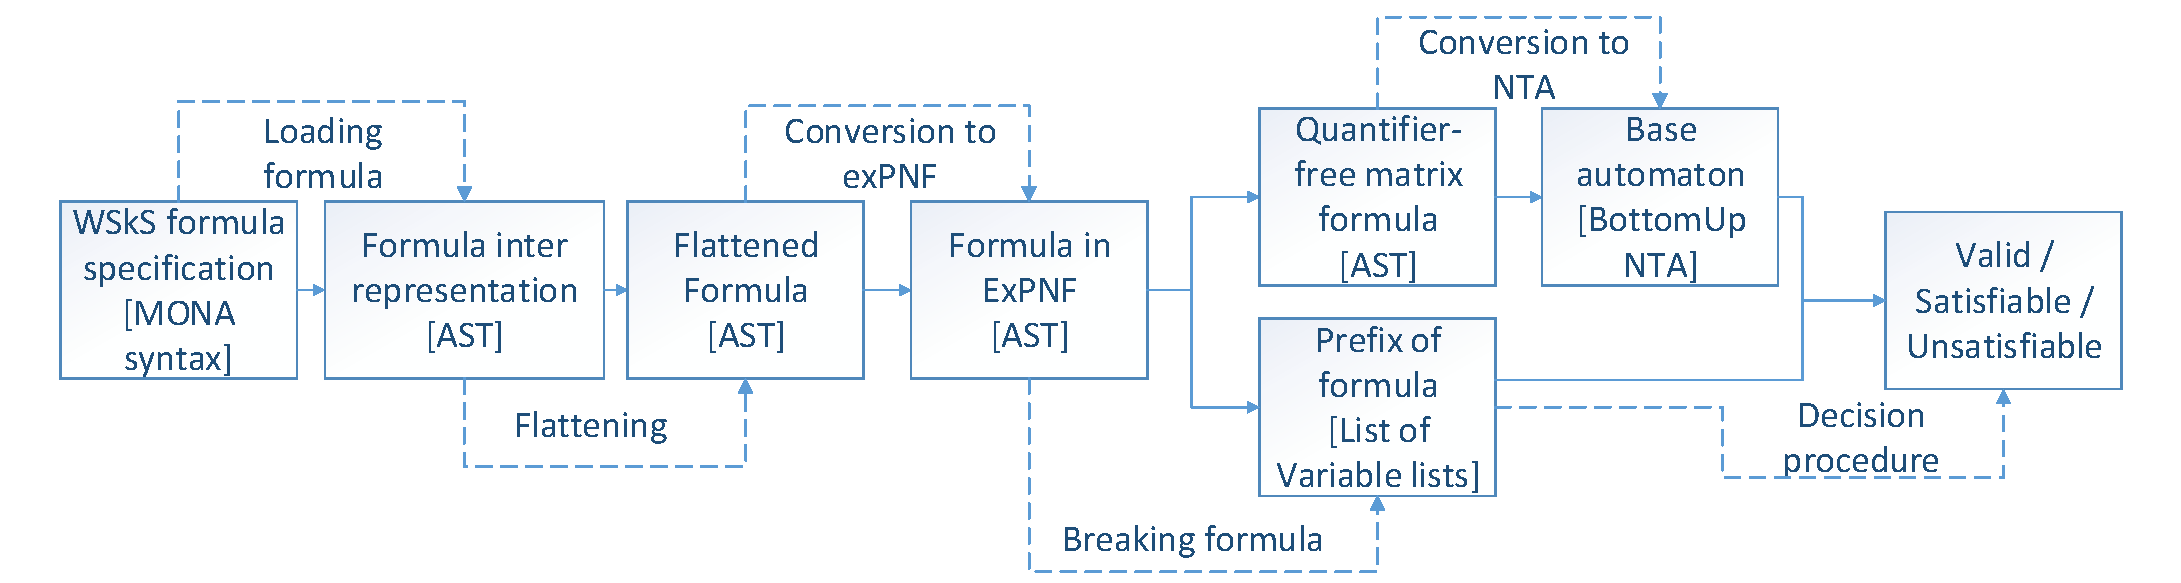
\includegraphics{fig/flow.pdf}}
 \caption{Transformation of data through the decision procedure}\label{flow}
 \end{center}
\end{figure}

\section{Manipulation with NTA}

For the representation of automata used in the decision procedure, the
\texttt{libvata} library~\cite{vata-tool}, written in C++, was chosen for being
an efficient and open source library that exploits some of the recent
developments of algorithms for NTA manipulation. Its main use is in the fields
of formal verification, but it can be efficiently used in other domains as well.

\texttt{libvata} supports two possible encodings of tree automata
(\emph{explicit} and \emph{semi-symbolic}) which differ in the way they store
the transition relations of automata. The semi-symbolic representation uses
MTBDDs for storing the transitions of automata as described in Section
\ref{mtbdd}. This is mostly intended for automata with large input alphabets
like in the case of some decision procedures of logics such as
WS$k$S~\cite{mona} or MSO~\cite{mso} (monadic second-order logic). The library
is designed in a~modular way, so it can be easily extended with new encodings
and operations.

The library provides a~command line interface, so the input of the library is
usually a~text representation in Timbuk format~\cite{timbuk}, which
is parsed and transformed into inner representation with states, transition,
alphabets, etc. However, we can also build the automaton from scratch using API
functions for appropriate encodings. Each automaton can be serialized back to an
output format (like Timbuk) through serializers.

We are going to use the semi-symbolic encoding that provides both bottom-up and
top-down representation of tree automata. These representation differs in
storage of MTBDD where for top-down representation the storage is more complex,
while on the other hand, in the bottom-up representation arity can be inferred
from the arity of the tuples on the left-hand side of the transition. As for the
representation of automata, we have chosen the bottom-up representation.

 \section{Decision procedure}
 \begin{algorithm}[h!]
		\SetKwFor{For}{foreach}{do}{}
		\SetKwRepeat{Repeat}{repeat}{until}
		\KwIn{A~state $I_m$ of the automaton $A_{\varphi_m}$, a~level of
		determinization $m$}
		\KwOut{\textsc{TRUE} iff $\varphi_m$ is valid, \textsc{FALSE} otherwise}
		\KwData{\texttt{StateCache} caches the answers of the \texttt{StateIsFinal}
		function}
		\BlankLine
		\nl\Return \texttt{IsStateFinal}($I_m$, $m$)\;
		\BlankLine
		\SetKwProg{myproc}{Function}{}{}
 		\myproc{\upshape \texttt{IsStateFinal}(\textbf{state} $P$, \textbf{level}
  $i$)}{ 
  		\nl $\mathit{isFinal}$ := \texttt{StateCache}[$P$, $m$]\;
  		\nl\uIf{$\mathit{isFinal}$ $\neq \bot$}{
  			\nl \Return $\mathit{isFinal}$\;
  		}
  		\BlankLine
  		\nl\uIf{m = 0}{
  		  \nl \Return $Q \in F_0$\;
  		}
  		\nl\Else{
  			\nl\For{$q \in Q$}{
  				\nl\uIf{\upshape \texttt{CheckForAcceptingState}($q$, $m \minus 1$)}{
  				    \nl \texttt{StateCache}[$P$, $m$] := \textsc{FALSE}\;
  					\nl\Return \textsc{FALSE}\;
  				}
  			}
  			\nl \texttt{StateCache}[$P$, $m$] := \textsc{TRUE}\;
  			\nl \Return \textsc{TRUE}\;
  		}
  }
		\caption{Implementation of deciding validity of WS$k$S formula
		}\label{impl-main}
	\end{algorithm}
 
 In Chapter \ref{our} we introduced the formal concepts of deciding WS$1$S
 with non-deterministic automata and designed the algorithm for testing
 validity of a~given formula $\varphi$. We then further extended this approach
 to an arbitrary $k$. In this section we will closely describe the practical
 implementation of this formal algorithm in the C++ language. The prototype of
 this procedure is going to be restricted to WS$1$S only.
 
 For each level $1 \leq i \leq m$ we define two caches that will store the
 already computed results to avoid their repeated computation during the
 decision procedure. In case we get a~cache miss, the value $\bot$ is returned
 instead. $\mathit{BDDCache}_i$ is a~cache that maps states of level $i$ to
 their corresponding MTBDDs representing their transition relations $\delta_i$, i.e.
 \begin{equation}
  \mathit{BDDCache}_i : Q_i \rightarrow ((\Sigma_i \rightarrow 2^{Q_i}) \cup
  \{\bot\}).
 \end{equation}
 
 Further we define the cache $\mathit{StateCache}_i$ for storing which states
 are final and which are non-final, i.e.
 \begin{equation}
  \mathit{StateCache}_i : Q_i \rightarrow \{Final, NonFinal, \bot\}
 \end{equation}
 
 The core function for deciding WS$k$S is \ref{impl-state-is-final} which checks
 whether there exists a~reachable final state on level $0 \leq i \leq m$ from
 state $q$. This function is corresponding to the implementation of Algorithm
 \ref{deciding-wsks-alg} with use of function \ref{impl-succ} for building successors of
 states and function \texttt{IsStateFinal} from Algorithm \ref{impl-main} for
 checking whether the state is final.
 The implementation is based on the workset algorithm and uses efficient apply
 operations over the MTBDDs of constructed successors.
 
\begin{function}[ht!]
		\SetKwFor{For}{foreach}{do}{}
		\SetKwRepeat{Repeat}{repeat}{until}
		\KwIn{A~state $q$ of the automaton $A_{\varphi_m}$, a~level of determinization
		$m$} \KwOut{\textsc{TRUE} if there is a~reachable accepting state from $q$,
		\textsc{FALSE} otherwise}
		\BlankLine
		\nl $\mathit{workset}$ := $\{q\}$\;
		\nl $\mathit{processed}$ := $\mathit{workset}$\;
		\nl \While{$\exists q_m \in workset$}{
			\nl $\mathit{workset}$ := $\mathit{workset}$ $\setminus \{q_m\}$\;
			\nl\uIf{\upshape \texttt{IsStateFinal}($q_m$, $m$)}{
				\nl \Return \textsc{TRUE}\;
			}
			\nl\Else{
				\nl $\mathit{succ}$ := \texttt{buildSuccessorTree($q_m$, $m$)}\;
				\nl\textbf{apply1} $\mathit{succ}$ ($\lambda$ x. \textbf{if} $x \notin
				\mathit{processed} \wedge \neg\exists y \in \mathit{processed}: x < y$ \\
				\hspace*{33mm}\textbf{then} $\mathit{workset}$ := $\mathit{workset}$ $\cup
				\{x\}$)\; \nl $\mathit{processed}$ := $\mathit{processed}$ $\cup$ $\mathit{workset}$\; 
				} 
			}
			\nl\Return \textsc{FALSE}\;
		\caption{CheckForAcceptingState(state $q$, level
		$m$)}\label{impl-state-is-final}
\end{function}
 
 The main Algorithm \ref{impl-main} for deciding WS$k$S is corresponding to the
 implementation of Algorithm \ref{universality}. It first checks the cache
 whether a~state has already been decided and else calls the
 function \ref{impl-state-is-final} for checking if there exists
 a~reachable final state.
 
 We can further extend this procedure to deciding satisfiability of WS$k$S
 formulae by~checking the validity of $\exists$-closed input formulae. This
 means that given the input we close the formula and its negation and test the
 validity of constructed formulae to decide their satisfiability. Further we can
 decide the formula according to the relationships between validity,
 satisfiability and unsatisfiability~\cite{logics}.
 
\begin{function}[h!]
		\SetKwFor{For}{foreach}{do}{}
		\SetKwRepeat{Repeat}{repeat}{until}
		\KwIn{A~state $q$ of the automaton $A_{\varphi_m}$, a~level of determinization
		$m$}
		\KwOut{A~successor of state $q$}
		\KwData{\texttt{BDDCache} mapping macro-states to their transition BDDs}
		\BlankLine
		\nl $\mathit{succ}$ := \texttt{BDDCache}[$q$]\;
		\nl \uIf{$\mathit{succ}$ $\neq \bot$}{
			\nl \Return $\mathit{succ}$\;
		}
		\nl $\mathit{succ}$ := $\emptyset$\;
		\nl\For{$r \in q$}{
			\nl $\mathit{childSucc}$ := \texttt{buildSuccessorTree}($r$, $m-1$)\;
			\nl \textbf{apply2} $\mathit{succ}$ $\mathit{childSucc}$ ($\lambda$ $x$ $y$. $x$ $\cup$ $y$)\;
		}
		\nl $\mathit{succ}$ := \texttt{project}($\mathit{succ}$,
		$\mathit{level}$)\; \nl \texttt{BDDCache}[$q$] := $\mathit{succ}$\;
		\nl \Return $\mathit{succ}$\;
		\caption{buildSuccessorTree(state $q$, level $m$)}\label{impl-succ}
	\end{function}
\newpage
 The successor of a~state can be constructed out of its children
 as described by the function \ref{impl-succ}.
 This construction is also optimized with the use of the cache. After the MTBDDs
 for transitions of children of a~state are built, we use the binary apply for doing
 the union of those MTBDDs to yield the MTBDD corresponding to the transition
 from the state. This MTBDD is further modified using the operation of
 projection.
 
 \section{Optimizations}\label{optimizations}
 
 During the implementation process we used the tool
 \texttt{valgrind}~\cite{valgrind}, especially its part \texttt{callgrind}, to
 profile the implementation in C++ and tried to identify weak spots of the
 application.
 One of the most frequent operations in the procedure are the relational
 operators on the classes representing macro-states used e.g. for pruning the
 state search, macro-state comparison and operations with worklist.
 
 We propose to optimize this by using bitwise operations and bit array for
 storing the leaf states to ease some of the computation. There are several
 possibilities to use in C++~\cite{bitwise} and we have chosen the container
 with best performance, which is \texttt{boost::dynamic\_bitset}. The results
 have shown that the performance of comparison between macro-states of first
 level of determinization got better by fair margin. 
 
 Besides some of the minor optimizations, we also extended the set of atomic
 formulae and tried to cache some of the intermediate results during the
 process to lessen the computation time. We will briefly describe these
 optimizations in the following subsections and the impact of the optimizations
 will be further discussed in following Chapter \ref{evalChapter}.
 
 \subsection{Extending set of atomic formulae}
 
 While the set of atomic formulae in the restricted syntax is indeed enough for
 defining the whole range of WS$k$S logic, automata corresponding to the
 flattened versions of some of atomic formulae (like $\leq$ for example) can
 be too large for processing and slow down the algorithm. As shown in Table
 \ref{atomic-formulae} we can heavily reduce the size of the matrix automaton
 just by extending the set of the atomic formulae defined in \ref{restricted} and
 construct special automata for frequently used operations and yielding
 smaller base automata in result. 
 
 \begin{table}
  \catcode`\-=12
 \begin{center}
  \begin{tabular}{|c|c|c|c|c|}
  \hline  
     \multirow{2}{*}{\textbf{Formula}}          
                    &\multicolumn{2}{c|}{\textbf{quantifiers}/\textbf{alternations}}&\multicolumn{2}{c|}{\textbf{automaton
                    size [states]}}\\
    \cline{2-5}
     & \textbf{before}     &    \textbf{after}    &
    \textbf{before}     &    \textbf{after}\\
    \hline
    \hline
    $X \subseteq \mathbb{N}$ & 0 & 0 & $\infty$ & max($X$)$ + 2$\\
    \hline
    $X = \{1, 4, 6\}$ & 0 & 0 & 24 & 8\\
    \hline
    $X = \{1, 3, 5, 7, 9\}$ & 0 & 0 & 93 & 11\\
    \hline
    \hline
    $x \in X$ & 0 & 0 & 5 & 2\\
    \hline
    const $k \in X$ & $k+1$ & 0 & $k$+3 & $k$+3\\
    \hline
    $0 \in X$ & 1 & 0 & 3 & 3\\
    \hline
    $1 \in X$ & 2 & 0 & 4 & 4\\
    \hline
    \hline
    $x \leq y$ & 3/2 & 0 & 13 & 4\\
    \hline
  \end{tabular}
 \end{center}
 \caption{Comparison of the basic set of atomic formulae with the extended set
 in size of the automaton, number of quantifiers and alternations. Note that $\infty$
 denotes that number of states cannot be measured or described by mathematical
 equation.}\label{atomic-formulae}
 \end{table}
 \newpage
 \noindent\hrulefill
 \begin{example}
 Let us take the formula $\varphi \overset{\mathit{def}}{=} x \leq y$ for
 example.
 In the classical restricted syntax, this formula $\varphi$ would be flattened as follows:
 \begin{equation}
  x \leq y \overset{\mathit{def}}{\Leftrightarrow} \forall X. (y \in X \wedge
  (\forall z.
  z1 \in X \Rightarrow z \in X)) \Rightarrow x \in X
 \end{equation} 
 which corresponds to the automaton with 13 states. However, we can construct
 the following atomic automaton with 4 states only depicted in Figure
 \ref{less-eq}, which means we can save around $70\%$ of states.
 \begin{figure}[h!]
 \begin{center}
  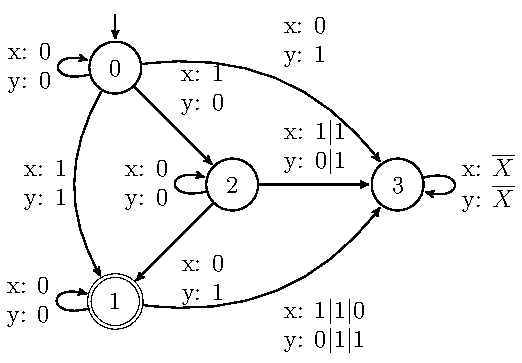
\includegraphics{fig/atomic-x-lesseq-y}
 \end{center}
 \caption{Atomic automaton corresponding to atomic formulae $x \leq
 y$}\label{less-eq}
\end{figure}
 \end{example}
 \noindent\hrulefill

 Even though some of the reductions can seem to be
 insignificant, due to their frequent occurrences in many practical formulae the
 overall reduction can be enormous in result. Another reduction comes from
 lessening the number of quantifications produced by creation of some temporary
 variables like for formula $\varphi \overset{\mathit{def}}{=} k \in X$ which
 after extending atomic formulae yields same number of states, however without
 quantifications, and hence decrease the number of projections of MTBDDs during
 the process.
 
 Besides defining automata for more of the WS$k$S syntax connectives and atomic
 formulae, we could extend the syntax even further and create some of the more
 complex operations like the modulo or the predecessor predicate, just like
 \textsc{MONA} does, which are not specifically defined in WS$k$S logic.
 \textsc{MONA}~\cite{mona-secrets} takes this even further and allows us to
 define external automata that can be included in the input specification.
 
 Note that we can decide Presburger formulae~\cite{presburger} with the basic
 set of atomic formulae as shown for example in~\cite{nfa}. This
 approach yields big automaton in process with one alternation of negation for
 each addition in formula. However, we can construct a~special automaton
 accepting the addition of two Presburger constants with 4 states only, thus
 greatly reducing the time needed to decide this family of formulae.
 
 \subsection{Cache}
 
 The caching of some of the intermediate products can be applied to several
 places in code. First we can cache the already computed results of deciding
 which of the macro-states are final or non-final. Also during the computation
 of successors of states, we can cache the MTBDDs that were already constructed
 before.
 
 Generally, caching is a~trade-off between time and space, which raises the
 questions how much will we store in the cache. One of the most frequent
 operations over MTBDDs is the union of posts of macro-states. By storing all of
 the intermediate results during the union of MTBDDs we can speed up the
 algorithm greatly on the expenses of using more memory.
  
 With the design of algorithm, which is looking for existing example, i.e.
 searching for reachable state, in automaton corresponding to the formulae and
 its negation (to get counterexample) this means we do not have to compute
 and classify lots of states twice.

\chapter{Evaluation}\label{evalChapter}

In this chapter we are going to provide an evaluation of our tool
\texttt{dWiNA}\footnote{\texttt{d}eciding \texttt{Wi}th
\texttt{N}on-deterministic \texttt{A}utomata}\,---\,an implementation of
the decision procedure described in the previous chapters.
All the tests were performed in a virtualized environment with the Linux Ubuntu 12.10 operating
system with 4\,096\,MB of operating memory and one virtual processor natively
running on a~laptop computer with 8\,GB RAM memory and a~dual core processor
running on 2.5\,GHz.

The performance of our prototype implementation was tested by measuring several
different metrics and compared with the \textsc{MONA} tool which uses the
deterministic tree automata instead of non-deterministic automata used in our
approach and is heavily optimized (See Section \ref{monasecrets}) as well.
The run tests were measuring the speed and size of the state space of
the decision procedure depending on the size of the input formula and the number
of quantifier alternations. The other tests were examining the impact of the
used optimizations on the performance of our implementation, like the cache hit-miss
ratio or the overall speed.

Note that we will use the symbol $\infty$ if either the test fails due to
insufficient memory or it has been interrupted due a timeout, which was set to 5
minutes.

\section{Parametric Horn formulae}

Experiments done with our implemented tool were carried out
on a specific parametric family of formulae in the following Horn form:
\begin{equation}\label{horn}
 \varphi_n \overset{\mathit{def}}{=} \exists X\forall x_1\ldots x_n.
 \bigwedge_{i = 1}^{n-1} (x_i \in X \Rightarrow x_{i+1} \in X)
\end{equation}

The formulae in this family are closed and valid and suitable for
our experiments since we can freely change the number of alternations in
the formulae and the size of the resulting automaton depending on the quantifier
prefix and the parameter $n$.
Also it was further discovered that \textsc{MONA} is able to only decide
formulae up to the value of $n = 15$ due to insufficient memory for storing
MTBDDs.
In results it is proposed by its authors that the logical approach designed
in~\cite{logic-approach} proves to be better for solving this kind of formulae
in contrary to the automata-based approach used by both \textsc{MONA} and
\texttt{dWiNA}. However, we will show that our algorithm and the used library
for manipulating non-deterministic automata~\cite{vata-tool} is far more memory
efficient with handling MTBDDs and has no problems deciding these formulae and
thus can fairly compete with the logical composition approach.

\section{Comparison with \textsc{MONA}}
We have run tests with the generated formulae of the form \ref{horn} for
the parameter $n$ ranging from $2$ to $50$ with various numbers of quantifier
alternations bounded by the value of $n$ ranging from $2$ to $9$ alternations
per formula.
The size of the base automaton (corresponding to the quantifier-free matrix) is heavily
dependent on the number of alterations in the formulae as depicted in Table
\ref{n-size}. Even number of alternations spawns one additional negation of the
base automaton which then results in the disjunction of formulae that is handled
as the union of automata. This way the automaton size is increasing heavily in
the relation with parameter $n$.

\begin{table}[h!]
\catcode`\-=12
 \begin{center}
  \begin{tabular}{| c | r | r |}
  \hline
   \multirow{3}{*}{\textbf{n}} & \multicolumn{2}{|c|}{\textbf{automaton}}\\
                               & \multicolumn{2}{|c|}{\textbf{[states]}}\\
   \cline{2-3}
   & \textbf{odd alternations} & \textbf{even alternations}\\
   \hline
   \hline
   3 & 18 & 30\\
   \hline
   4 & 27 & 144\\
   \hline
   5 & 36 & 648\\
   \hline
   6 & 45 & 3~240\\
   \hline
   7 & 54 & 15~336\\
   \hline
  \end{tabular}
 \end{center}
 \caption{The base automaton size depending on the number of alternations in
 the formula and parameter $n$. The number of alternations can range
 from 1 to $n$, where even number spawns additional negation and
 results into the union of automata which heavily increases the
 resulting base automaton size.}\label{n-size}
\end{table}

In~\cite{logic-approach} it was proposed that this type of formulae is not
suitable for automata-based approach and logical decomposition is a much better
decision procedure. The results in~Table \ref{n=1} certainly proved that
\textsc{MONA} has problems with deciding these formulae for $n \geq 15$,
however, this is due to the enormous size of MTBDDs representing transitions in
the automatona that are stored as an optimization and not a~flaw in the
automata-based approach, since our tool \texttt{dWiNA} has no problems with deciding formulae
for a~greater $n$.

\begin{table}[h!]
\catcode`\-=12
\begin{center}
 \begin{tabular}{| r | r | r | r |}
 \hline
  \multirow{2}{*}{\textbf{n}}& \multicolumn{3}{| c |}{\textbf{time [s]}} \\
 \cline{2-4}
   & \textbf{logic} & \texttt{dWiNA} & \texttt{MONA}\\
  \hline
   \hline
  10 & 0.01 & 0.01 & 0.12\\
   \hline
  12 & 0.01 & 0.01 & 0.89\\
   \hline
  13 & 0.01 & 0.01 & 2.28\\
   \hline
  14 & 0.01 & 0.01 & 5.53\\
   \hline
  15 & 0.01 & 0.02 &15.06\\
   \hline
  16 & 0.01 & 0.02 & $\infty$\\
   \hline
  50 & 0.01 & 0.07 & $\infty$\\
  \hline 
 \end{tabular}
 \caption{Time evaluation of deciding formulae of the form \ref{horn} in
 dependence on the parameter $n$ for a fixed number of alternations
 (1).}\label{n=1}
 \end{center}
\end{table}

\begin{figure}[h!]
 \begin{center}
  \scalebox{0.47}{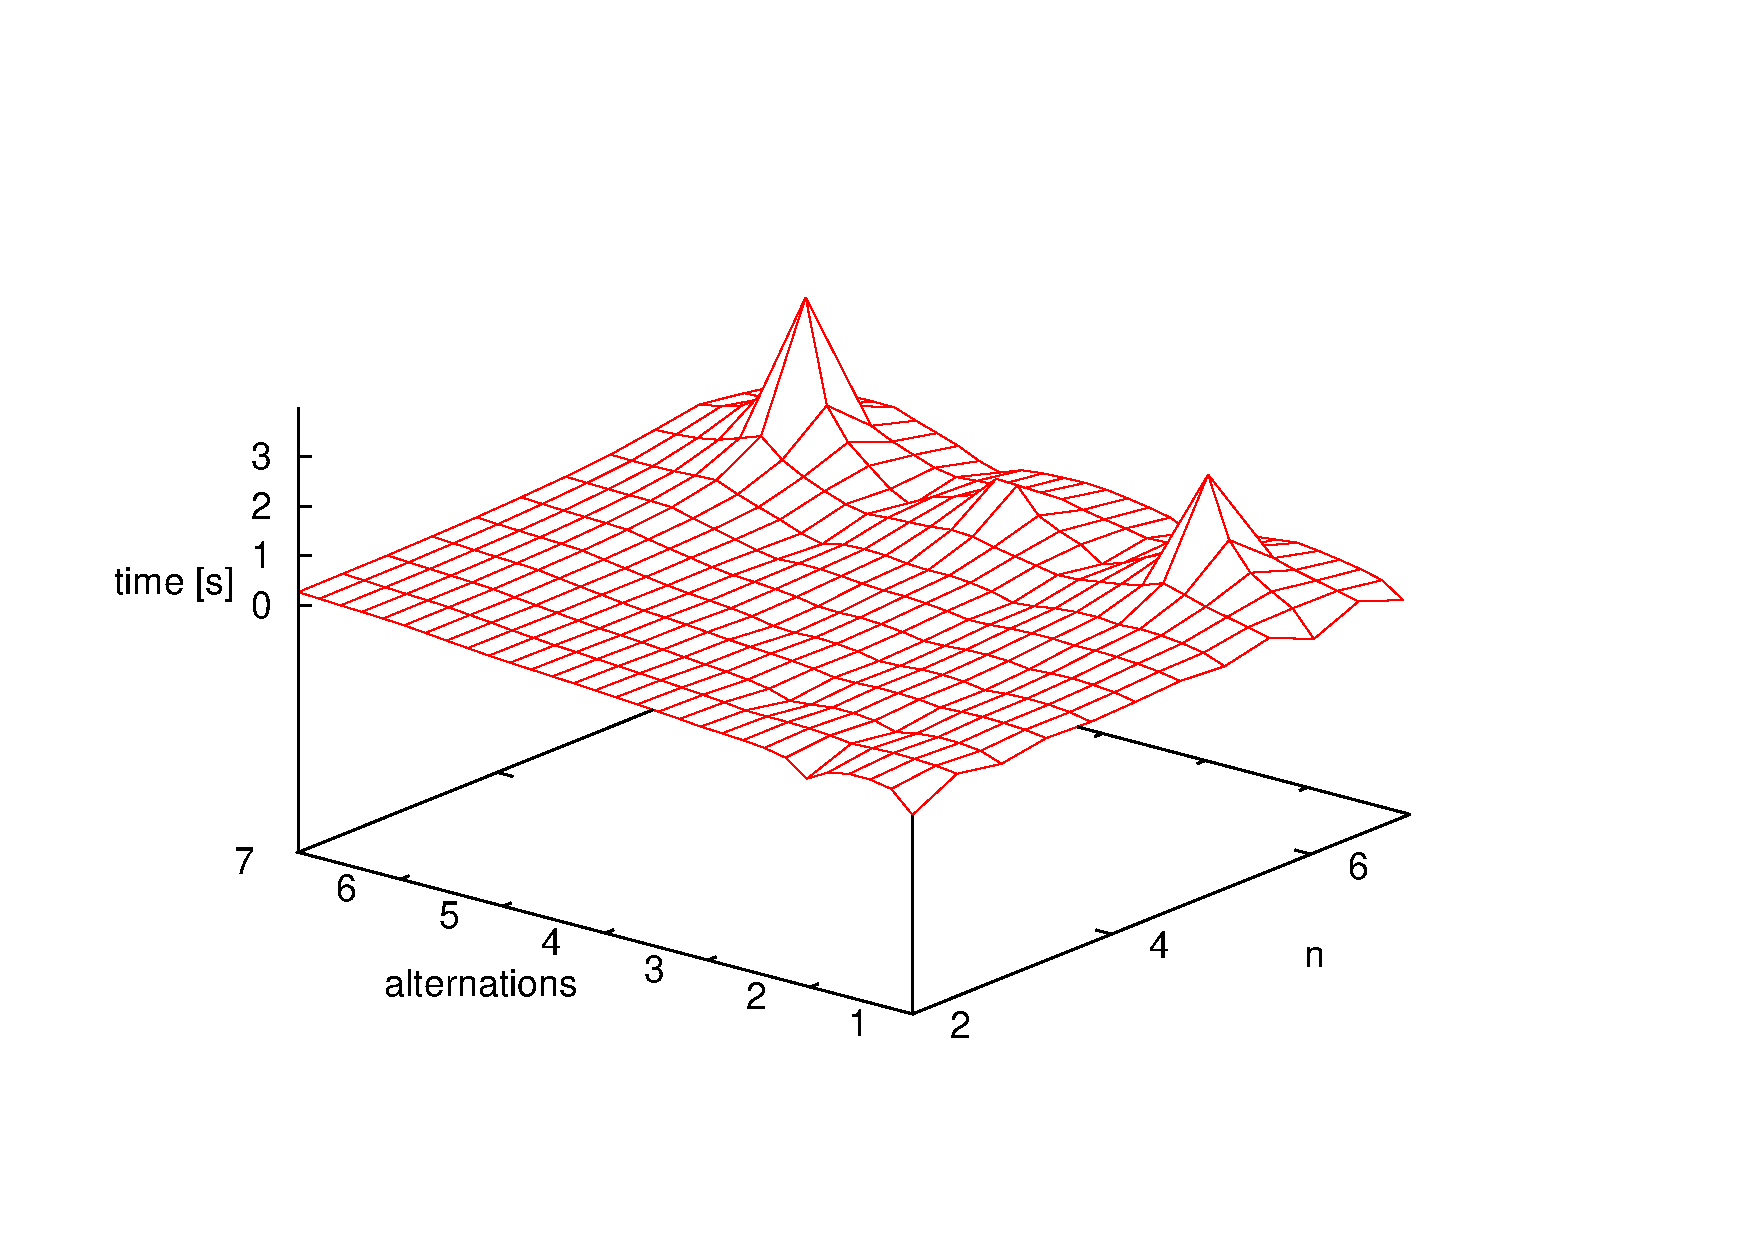
\includegraphics{fig/graf-alt-n-time}}
 \end{center}
 \caption{Speed performance of \texttt{dWiNA} based on
 the parameter $n$ and the number of alternations in the formula. For
 even number of alternation the size of the base automaton rises
 heavily and thus increases the overall time needed to perform the
 decision procedure.}\label{alt-n}
\end{figure}
\newpage
We further compared our tool with the \textsc{MONA} tool in dependence on the
parameter $n$ and the number of alternations. It is clear from Figure
\ref{alt-n} that due to the huge differences in the base automaton size between
odd and even alternations on the generated benchmark formulae the time needed
for the computation is rather unsteady for our implementation. This is because
of the inefficient representation of macro-states which makes some operations
take too much time to compute, like pruning or state comparison. \textsc{MONA},
however, has no problem with alternations and yields steady times for all numbers of
alternations showing that the full construction of the automaton along with
minimizations is still efficient and gives good results. This is contrary to our base
assumption that our \emph{on-the-fly} approach should not have issues with
alternations. Note that some combinations of alternations and parameter $n$
cannot be done and were thus approximated in the shown mesh grid.

\begin{table}
\begin{center}
 \begin{tabular}{|c|r|r|}
  \hline
  \textbf{alternations} & \texttt{dWiNA} & \textsc{MONA}\\
  \hline
  \hline
  2 & 2.20 & 0.01\\
  \hline
  3 & 0.01 & 0.01\\
  \hline
  4 & 1.49 & 0.01\\
  \hline
  5 & 0.04 & 0.01\\
  \hline
  6 & 2.90 & 0.01\\
  \hline
 \end{tabular}
 \end{center}
 \caption{Time comparison of \texttt{dWiNA} and \textsc{MONA} with fixed $n =
 6$}
\end{table}
\newpage
In Figure \ref{size-n} we show the alternate view on the data: the time
comparison with \textsc{MONA} based on the size of the base automaton (our).
Here we see that in dependence on the size of the automaton our approach is not
that bad and can yield good results even though there are no automata reductions during the
process. Even though \textsc{MONA} is far more consistent when it comes to the number of
alternations of quantifiers in the formulae and has better computational
results, in terms of the generated and evaluated search space our \texttt{dWiNA}
is more efficient. Figure \ref{state-graph} shows that the \emph{on-the-fly}
approach generates much less states and needs only a~portion of them for evaluation. This
shows that our approach certainly has a~potential to beat \textsc{MONA} even in
time, but requires additional optimizations to take place.

\begin{figure}[h!]
 \begin{center}
  \scalebox{0.6}{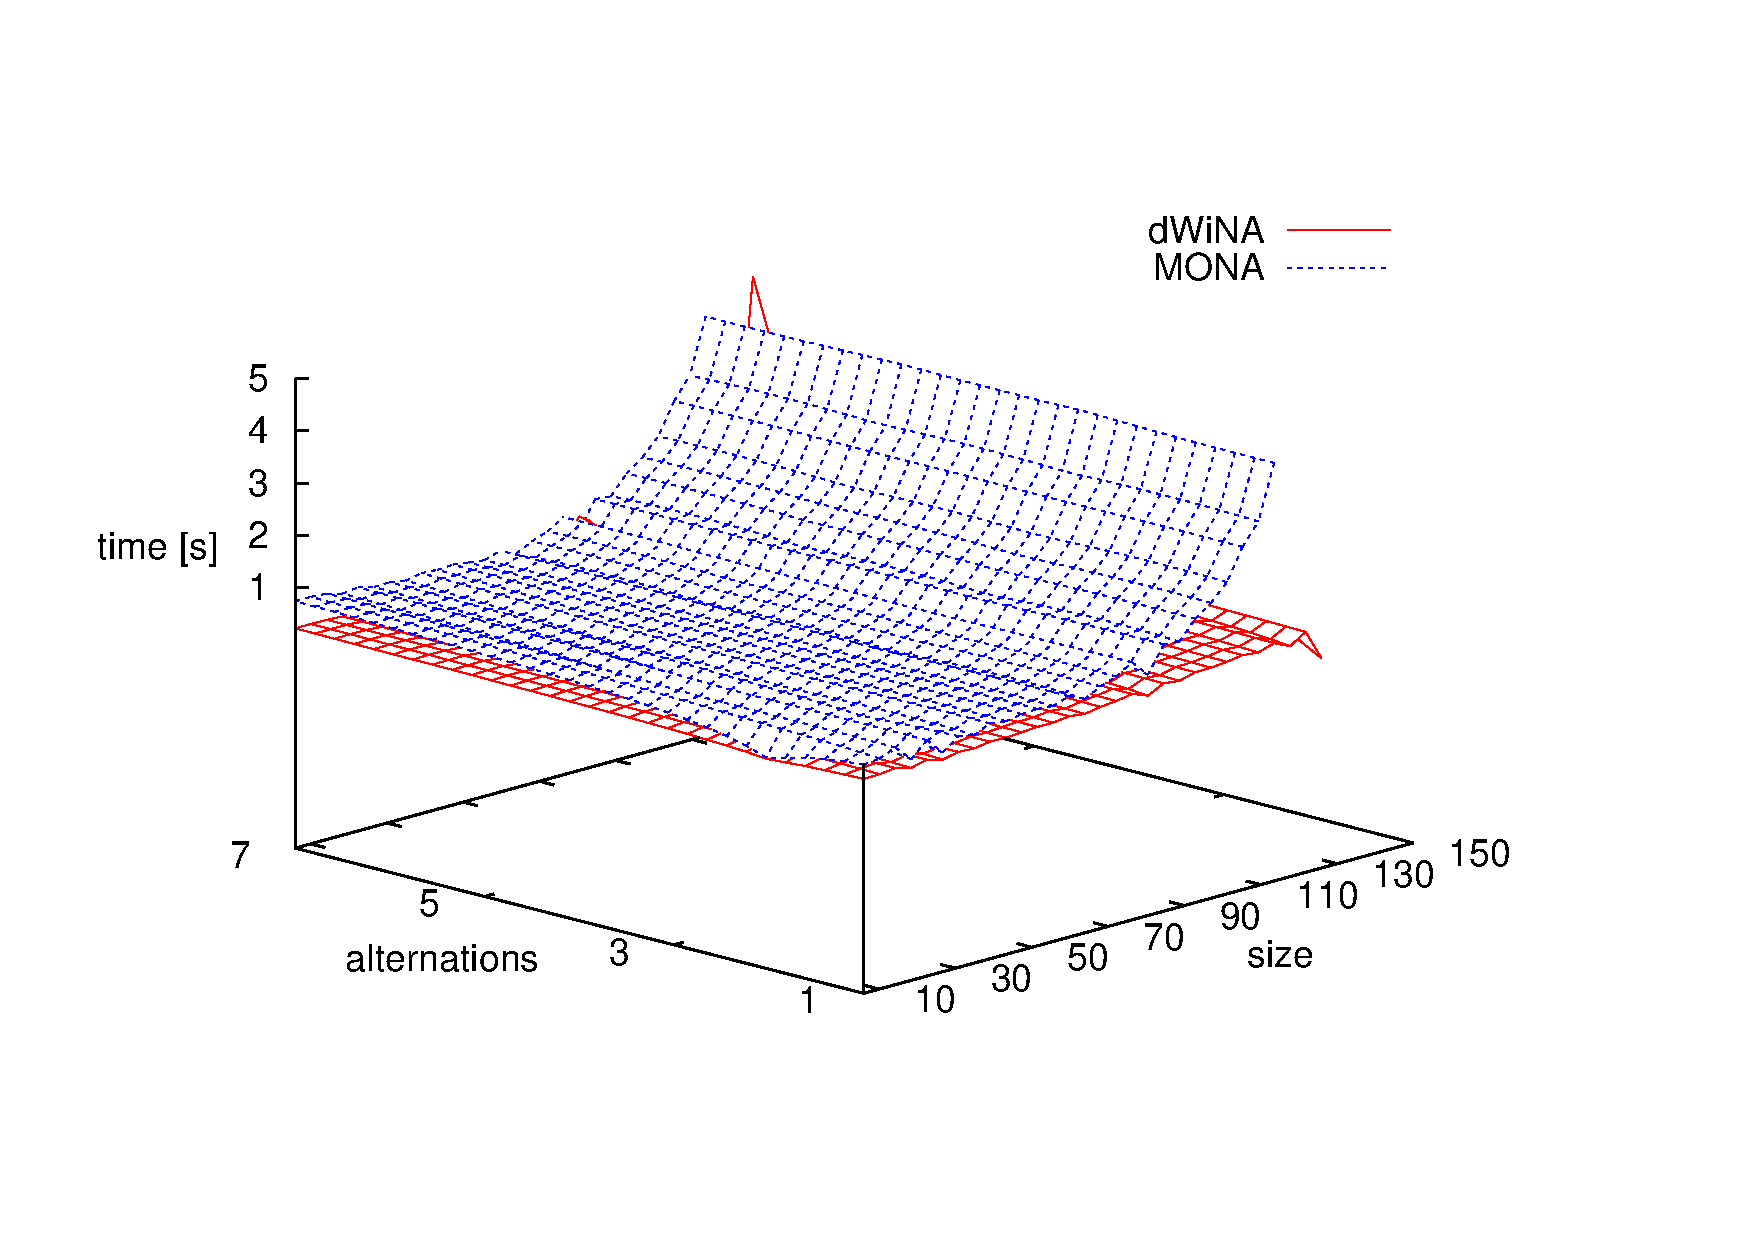
\includegraphics{fig/graf-alt-size}}
 \end{center}
 \caption{Alternative speed comparison of \texttt{dWiNA} and \textsc{MONA}
 based on the size of the automaton.}\label{size-n}
\end{figure}

\begin{figure}[h!]
 \begin{center}
  \scalebox{0.6}{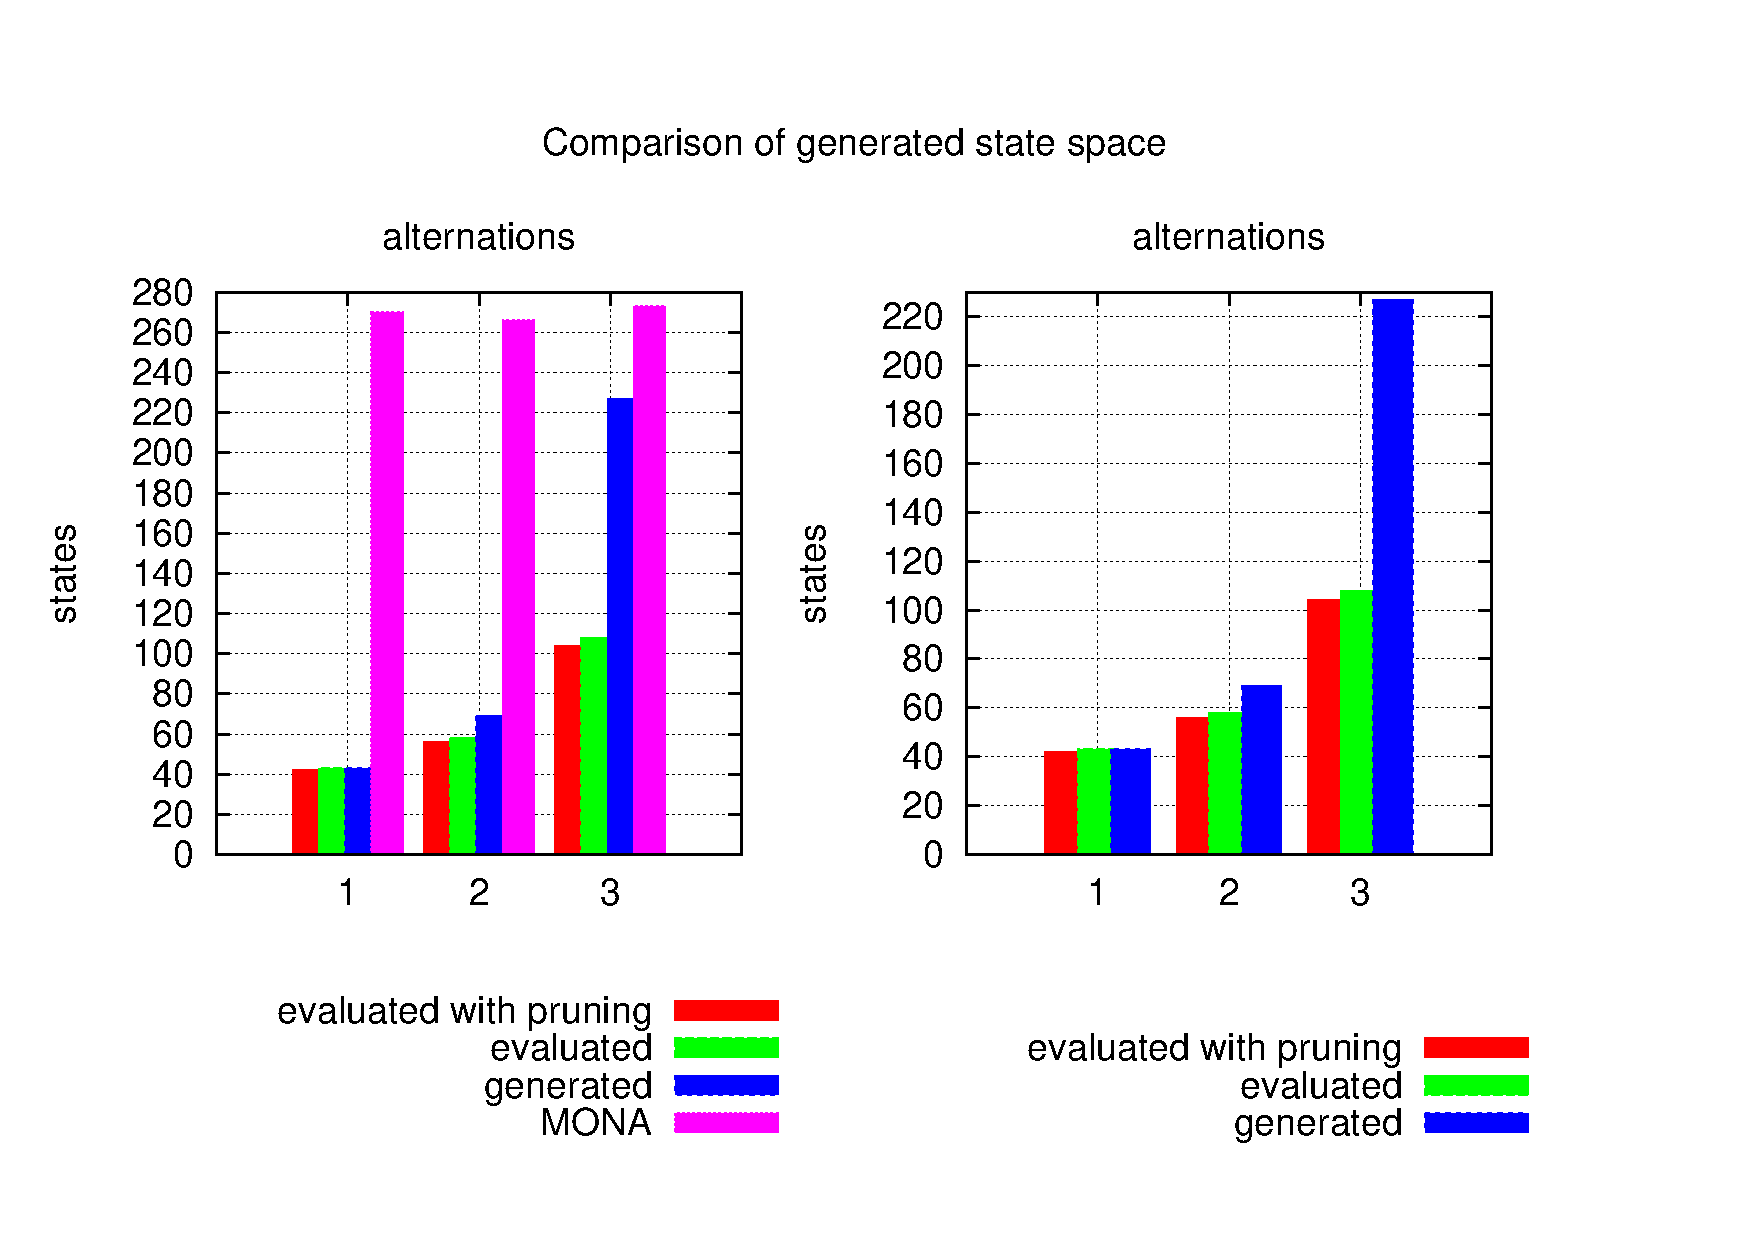
\includegraphics{fig/graf-states}}
 \end{center}
 \caption{Comparison of the number of the generated/evaluated states between
 \texttt{dWiNA} and \textsc{MONA} on the base automaton with $36$
 states.}\label{state-graph}
\end{figure}
\newpage
The other thing is that for many practical cases we do not need the fully
expanded automaton to decide whether its language is universal (or empty) and usually any
non-accepting (or accepting) suffices. Thus the \emph{on-the-fly} approach is
more suited for these kinds of problems.

\section{The impact of the used optimizations}

We will discuss the impact of optimizations developed
on the performance of the implementation. Aside from some minor
optimizations we introduced some of our implementation secrets in Section \ref{optimizations}.
The most notable ones is the pruning of the states during the search for the
accepting states. The other ones is smarter flattening of the input formulae
with an~extended set of atomic formulae and the caching during the process.

We can see from Table \ref{opt-times} that all of these optimizations have a
great impact on the performance. However, the greatest one is definitely the
smart flattening since this way we are working with considerably smaller automata than
with the basic atomic automata set. The pruning of the state space had a lower
impact on this kind of formulae than expected as shown in Figure
\ref{state-graph}, but still is a~great asset to the overall speed.

\begin{table}[h!]
\catcode`\-=12
 \begin{center}
  \begin{tabular}{| r | c || r | r | r | r | r |}
  \hline
   \textbf{n} & \textbf{alternations} & \textbf{all [s]} & \textbf{no opt
   [s]} & \textbf{pruning [s]} & \textbf{smart flatten [s]} & \textbf{cache
   [s]}\\
   \hline
   \hline
    \multirow{4}{*}{5} & 2 & 0.11 & $\infty$ & 24.05 & 0.49 & 25.20\\
    \cline{2-7}
     & 3 & 0.02 & 0.75 & 0.16 & 0.04 & 0.08\\
    \cline{2-7}
     & 4 & 0.14 & $\infty$ & $\infty$ & 1.09 & 13.71\\
    \cline{2-7}
     & 5 & 0.03 & 5.40 & 1.04 & 0.17 & 0.42\\
    \hline
   \hline
   \multirow{4}{*}{6} & 2 & 2.20 & $\infty$ & $\infty$ & 9.59 & $\infty$\\
   \cline{2-7}
    & 3 & 0.01 & 1.22 & 0.30 & 0.06 & 0.14\\
    \cline{2-7}
    & 4 & 1.49 & $\infty$ & $\infty$ & 11.15 & $\infty$\\
    \cline{2-7}
    & 5 & 0.04 & 17.7 & 2.34 & 0.28 & 2.47\\
   \hline
  \end{tabular}
 \end{center}
 \caption{Speed comparison for various optimizations based on the number of
 alternations and the parameter $n$. The columns show what
 optimization was used with implementation and time it took to
 decide the given formula.}\label{opt-times}
\end{table}
\newpage
Other notable optimization is definitely the cache. Based on the result in
Table \ref{opt-times} the impact of caching intermediate results during the
decision process is high and for some $n$, where the implementation
without optimizations fails, is even able to give a proper answer. While
the cache that stores whether a given state is final or non-final is not overly
used in~the process, the cache for storing MTBDDs and especially some of the
intermediate results during the construction of MTBDDs corresponding to the
successors of states is used in~more than $75\%$ of cases. A more detailed
look on the efficiency of the MTBDD cache is depicted in Table \ref{cache-hits}.
The cache was tested on various formulae of the parameter $n$ and the results
are shown for macro-state levels up to $7$.

\begin{table}[h!]
 \begin{center}
  \begin{tabular}{| r | r |}
  \hline
   \textbf{Level} & \textbf{Cache-hit ratio}\\
   \hline
   \hline
   1 & 0.816\\
   \hline
   2 & 0.768\\
   \hline
   3 & 0.760\\
   \hline
   4 & 0.728\\
   \hline
   5 & 0.704\\
   \hline
   6 & 0.667\\
   \hline
  \end{tabular}
 \end{center}
 \caption{Average cache-hit ratio for various level of determinizations for
 the MTBDD cache.}\label{cache-hits}
\end{table}

\section{Discussion of results}

In this chapter we have shown that the implementation can beat
\textsc{MONA} in several aspects, namely the generated search space and for some
cases the computation time to decide benchmark formulae. While \textsc{MONA} is
indeed far more consistent with its results, we can see that for some kinds of
formulae generating the whole state space can be excessive and to search for an
accepting state in the automaton corresponding to formulae only a small fragment
of the state space is required. 

Our tool thus has a~good potential of becoming a proper decision procedure for
WS$k$S, but still needs some optimizations to yield more consistent results in practice. 

\chapter{Conclusion}\label{summary}

In this work we introduced the WS$k$S logic and some of its decision procedures
and implementations.
We have described the classical approach that uses deterministic automata, as well
as the \textsc{MONA} tool that enhances this procedure by using several
optimizations and discussed their complexity issues and problems they have to deal with.

Another approach was proposed that uses non-deterministic automata instead of
deterministic ones. This makes use of recent developments in fields of
non-deterministic automata algorithms, like universality checking or language
inclusion, allowing us to implement a~procedure similar to antichain-based
testing~\cite{tacas} and search for rejecting or accepting states on-the-fly
without need to construct the automaton corresponding to the given formula at
all.

We implemented a~prototype of the designed decision procedure that is able to
handle a~subset of WS$k$S formulae, namely formulae for $k = 1$, and
studied the impact of the use of non-deterministic automata on several case
studies. Out of the computational results on a set of formulae we identified
some of the weak spots of the application and tried to optimize them to achieve
better results.

We evaluated our tool \texttt{dWiNA} on a family of parametric formulae of
the Horn form and compared it with \textsc{MONA} in several different aspects.
We have shown that the \emph{on-the-fly} approach generates only a~portion of
the state space in contrary to the classical deterministic approach. While
\textsc{MONA} is more consistent with its results and has no problems with
an excessive number of alternations, based on the size of the base automaton we
were able to beat \textsc{MONA} even in the speed. The non-deterministic
approach to deciding WS$k$S has indeed a~great potential and may yield good results with future research.

We further propose some optimizations that could
enhance the results. One of the weak spots of the implementation is
the size of the base automaton corresponding to the quantifier-free matrix
of the formula.
\textsc{MONA} always performs minimization after every operation so it works
with the smallest automata possible. We could reduce the size of non-deterministic
automata through simulation computation followed by the downward reduction. 

Most of the formulae used in practice share very similar subformulae that can be
represented as a single state and reuse the constructed automaton by reindexing
its variables. We propose to optimize the frontend of the procedure to use the
Direct Acyclic Graph (DAG) instead of plain AST. 

%=========================================================================
